\documentclass[10pt,a4paper]{article}

% Typography — OpenAI / Anthropic technical-report style
\usepackage[utf8]{inputenc}
\usepackage[T1]{fontenc}
\usepackage[english]{babel}
% Latin Modern: full Type1 (T1) outlines for roman, sans, typewriter and math.
% Fixes the Computer Modern *bitmap* (Type 3) fallback that fontenc T1 triggered
% in this TeX install and which garbled \texttt identifiers (e.g. the Algorithm
% listing) and made dense paragraphs look smeared. (Times/Helvetica/Courier
% metrics are not installed in this minimal TeX; Latin Modern is and looks the
% same as Computer Modern but renders as crisp vector outlines.)
\usepackage{lmodern}
% With Type1 fonts, microtype font-expansion works and tightens justification.
\usepackage[protrusion=true,expansion=true]{microtype}
% Keep "--" / "---" as literal hyphens inside \texttt (CLI flags like
% --nthreads, --tile-sync, and compiler flags -O3 -flto ...). Without this the
% typewriter font renders "--" as an en-dash, corrupting any command
% copy-pasted from the PDF.
\DisableLigatures{encoding = *, family = tt*}
\usepackage[margin=2.5cm,top=2.2cm,bottom=2.5cm]{geometry}

% Block paragraphs (OpenAI / Anthropic technical-report style): vertical
% spacing between paragraphs instead of a first-line indent. Adds the
% "line breaks" / breathing room between paragraphs across the document.
\usepackage{parskip}

% Relax line-breaking to reduce overfull \hbox from long \texttt{...}
% identifiers that LaTeX cannot hyphenate.
\sloppy

% Math + symbols
\usepackage{amsmath,amssymb,amsfonts}
\usepackage{siunitx}
% Euro sign via textcomp (\texteuro): unlike eurosym's \euro, this carries a
% correct Unicode mapping, so "EUR500" copy-pastes as "\euro 500" not "e500".
\usepackage{textcomp}
\providecommand{\euro}{}\renewcommand{\euro}{\texteuro}

% Floats, tables, lists
\usepackage{booktabs}            % horizontal rules \toprule \midrule \bottomrule
\usepackage{tabularx}
\usepackage{multirow}
\usepackage{float}
\usepackage{graphicx}
\graphicspath{{figures/}}
\usepackage{enumitem}
% Bullet/numbered lists: clear left indent, room to breathe above/below the
% list and between items, and continuation lines aligned under the item text.
\setlist{leftmargin=1.6em,labelsep=0.6em,itemsep=4pt,topsep=6pt,parsep=0pt}
\setlist[itemize]{label=\textbullet}

% Graphics + diagrams
\usepackage{xcolor}
\usepackage{tikz}
\usepackage{pgfplots}
\pgfplotsset{compat=1.18}
\usetikzlibrary{shapes,arrows,positioning,fit,backgrounds,decorations.pathreplacing}

% Captions — small, italic, no colour
\usepackage[font=small,labelfont=bf,labelsep=period,justification=justified]{caption}

% Hyperref — blue links (OpenAI system-card style); colour set after xcolor below
\usepackage[breaklinks=true,bookmarks=true,bookmarksopen=true,unicode=true]{hyperref}

% Code listings — minimal, monospace, no background
\usepackage{listings}
\usepackage{verbatim}
\lstset{
  basicstyle=\ttfamily\footnotesize,
  frame=single,
  framerule=0.3pt,
  rulecolor=\color{black!40},
  breaklines=true,
  showstringspaces=false,
  language=bash,
  aboveskip=8pt,
  belowskip=8pt,
  xleftmargin=4pt,
  xrightmargin=4pt,
}

% Subtle figure/table accent (kept neutral, no decorations)
\definecolor{primary}{RGB}{30,30,30}
\definecolor{accent}{RGB}{160,55,30}
\definecolor{ok}{RGB}{40,120,60}
\definecolor{warn}{RGB}{170,120,30}
\definecolor{err}{RGB}{150,40,40}
\definecolor{codebg}{RGB}{248,248,248}

% Blue hyperlinks (OpenAI system-card style)
\definecolor{linkblue}{RGB}{0,0,190}
\hypersetup{colorlinks=true,linkcolor=linkblue,citecolor=linkblue,urlcolor=linkblue}

% Section headings — clean bold, no colour (OpenAI/NeurIPS style)
\usepackage{titlesec}
\titleformat{\section}{\large\bfseries}{\thesection}{0.8em}{}
\titleformat{\subsection}{\normalsize\bfseries}{\thesubsection}{0.6em}{}
\titleformat{\subsubsection}{\normalsize\itshape}{\thesubsubsection}{0.5em}{}
% \paragraph as a real heading on its own line (not run-in): turns the
% "Construct validity", "Internal validity", "Stage 13 ..." leads into
% visible sub-headings throughout the document, breaking up dense prose.
\titleformat{\paragraph}[hang]{\normalsize\bfseries}{}{0pt}{}
\titlespacing*{\section}{0pt}{14pt}{6pt}
\titlespacing*{\subsection}{0pt}{10pt}{4pt}
\titlespacing*{\paragraph}{0pt}{9pt}{3pt}

% Title block — centred, no rules, NeurIPS/OpenAI style
\usepackage{titling}
\pretitle{\begin{center}\Large\bfseries}
\posttitle{\par\end{center}\vspace{-0.4em}}
\preauthor{\begin{center}\normalsize}
\postauthor{\par\end{center}\vspace{-0.4em}}
\predate{\begin{center}\small\itshape}
\postdate{\par\end{center}}

% Abstract environment — clean centred heading, modest inset, no heavy quote
\renewenvironment{abstract}{%
  \vspace{2pt}\begin{center}\textbf{Abstract}\end{center}\par\vspace{1pt}%
  \begingroup\small\setlength{\leftskip}{1.8em}\setlength{\rightskip}{1.8em}\noindent\ignorespaces
}{%
  \par\endgroup\vspace{10pt}%
}

\title{Pushing Four Raspberry Pis to the Memory Wall:\\[0.15cm]
       Bit-Exact 30B Mixture-of-Experts Inference, $+$16\% over the Public Record}
\hypersetup{pdftitle={Pushing Four Raspberry Pis to the Memory Wall: Bit-Exact 30B Mixture-of-Experts Inference, +16\% over the Public Record},pdfauthor={Daniel Correa Villa}}
\author{Daniel Correa Villa\\
  \small HELLOMATIK.COM --- Raspberry Pi Cluster Lab}
\date{23 May 2026}

\begin{document}

% ---- Title page (system-card style: title alone, page 1) ----
\thispagestyle{plain}
\vspace*{3.5cm}
\begin{center}
  {\LARGE\bfseries Pushing Four Raspberry Pis to the Memory Wall\par}
  \vspace{0.4cm}
  {\large Bit-Exact 30B Mixture-of-Experts Inference,\\[0.15cm]
   $+$16\% over the Public Record\par}
  \vspace{1.8cm}
  {\LARGE\bfseries Daniel Correa Villa\par}
  \vspace{0.5cm}
  {\LARGE\bfseries HELLOMATIK.COM\par}
  \vspace{0.2cm}
  {\large Raspberry Pi Cluster Lab\par}
  \vspace{0.6cm}
  {\small\href{https://hellomatik.com/research/hitting-the-memory-wall-30b-moe-raspberry-pi}{\texttt{hellomatik.com/research/\allowbreak hitting-the-memory-wall-30b-moe-raspberry-pi}}\par}
  \vspace{1.6cm}
  {\small 23 May 2026\par}
\end{center}
\newpage

% ---- Table of contents (page 2) ----
\setcounter{tocdepth}{2}
\tableofcontents
\newpage

\begin{abstract}
A 30-billion-parameter Mixture-of-Experts language model (Qwen3-30B-A3B) runs on four Raspberry Pi~5 boards --- roughly \euro500 of CPU-only hardware, with no GPU or NPU --- at 15.143~tok/s decode, bit-exact. On \emph{identical} 16~GB silicon this is \textbf{+15.2\%} over the vanilla \texttt{distributed-llama} baseline (13.15~$\to$~15.143~tok/s, $n$=20) --- a confound-free figure that isolates the source-level and runtime-configuration work reported here. It is also \textbf{+16.1\%} above the highest publicly documented configuration for this model and hardware class (13.04~tok/s; b4rtaz~\#255, 8~GB SKU); we show that cross-SKU comparison carries no measurable hardware confound, since vanilla \texttt{distributed-llama} on our 16~GB cluster measures 13.15~tok/s --- within run-to-run noise of the 8~GB record.

We report the design, optimisation and rigorous benchmarking of a four-node Raspberry Pi~5 (16~GB) cluster for distributed inference of this Mixture-of-Experts (MoE) model (3B active parameters per token, top-8 of 128 experts) over Gigabit Ethernet.

After exhausting framework alternatives infeasible on ARM Linux without GPU/NPU acceleration (EXO requires Apple MLX; prima.cpp hangs on ZMQ topology discovery; llama.cpp RPC regresses 25$\times$), we adopt \texttt{distributed-llama} v0.16.5 with twelve source-level changes developed in this work --- eight framework patches and four bit-exact kernel and op-fusion optimisations --- plus persistent runtime kernel tuning. Every optimisation stage is individually validated bit-exact (SHA-256 of the generated token-id sequence against a fixed reference at \texttt{seed=42}, \texttt{temperature=0}).

The trajectory runs from a 5.70~tok/s Llama-3.1-8B dense baseline, through an 11.40~tok/s Qwen3-MoE baseline, to the 15.143~tok/s decode result above ($n$=20, 95\% CI $\pm$0.097), measured with the exact \#255 command (\texttt{nTokens=109} on every run); end-to-end sustained serving throughput, prefill included, is 14.449~tok/s.

ARM PMU profiling locates the residual bottleneck in LPDDR4X memory bandwidth (49\% backend-stalled cycles, 11.4~GB/s sustained per node of an approximate 17~GB/s ceiling). We catalogue twenty-six unsuccessful configurations, document the constraint-discovery process (strict bit-exact, no kernel rebuild, no model change, no overclock) that narrowed the design space, and find that co-located observability agents (Grafana Alloy, cAdvisor) tax this memory-bound decode by 5.18\% while leaving compute-bound prefill unchanged --- a clean, same-hardware confirmation that decode is bandwidth-bound.

The cluster reaches the memory wall of the Raspberry Pi~5; the single remaining bit-exact software lever is Async Tensor Parallelism, an estimated 250~LOC integration on the Phase~B foundation already shipped in the repository.
\end{abstract}

\begin{table}[h]
\centering
\small
\caption{Results at a glance.}
\begin{tabular}{@{}lr@{}}
\toprule
\textbf{Decode throughput} (apples-to-apples vs.\ the public ceiling) & \textbf{15.143 tok/s} \\
\quad improvement over b4rtaz~\#255 (13.04 tok/s, decode) & \textbf{+16.1\%} \\
\quad improvement over vanilla on identical 16\,GB silicon (confound-free) & \textbf{+15.2\%} \\
Sustained serving throughput (prefill included) & 14.449 tok/s \\
Time-to-first-token (TTFT) & 557 ms \\
Per-node DRAM bandwidth (sustained / vendor ceiling) & 11.4 / 17 GB/s \\
Hardware / cost & 4$\times$ Pi~5 16GB\, /\, $\sim$\euro500 \\
Telemetry-off gain on decode (paired A/B) & +5.18\% \\
Constraints honoured & bit-exact, no overclock, no model change \\
\bottomrule
\end{tabular}
\end{table}

\section{Introduction}

Edge inference of large language models on consumer single-board computers (SBCs) is increasingly studied as a privacy-preserving, low-cost alternative to cloud inference \cite{geerling2025,stratosphere2025}. The Raspberry Pi~5 is the most widely deployed ARM-based SBC with enough RAM (16~GB) to host 8B-parameter quantised models, and its Ethernet I/O allows small clusters to be formed.

The absence of a usable GPU --- the VideoCore VII lacks general compute shaders --- restricts inference to the CPU, where execution is memory-bandwidth-bound.

\paragraph{Investigation timeline at a glance.}
The investigation comprised three intertwined tracks:
\begin{enumerate}[label=(\roman*),leftmargin=2.2em]
  \item \textbf{Architectural exploration} (framework, model, quantisation): converged on \texttt{distributed-llama} + Qwen3-30B-A3B Q40, establishing the operational baseline of 11.40~tok/s.
  \item \textbf{Production-branch source work} (Stages~1--8, 7.18 $\to$ 13.720~tok/s): driven mainly by the Stage~4 switch from Llama~3.1~8B to Qwen3-MoE ($+$59\%), plus the F0/F1/F2 \texttt{distributed-llama} patches.
  \item \textbf{Bit-exact refinement} (Stages~9--15, 13.720 $\to$ 14.449~tok/s sustained; 15.143~tok/s decode): documented in detail here.
\end{enumerate}

\noindent Five hard constraints, discovered progressively and adopted as design rules, frame the entire work:
\begin{itemize}
  \item \emph{Bit-exact output} --- SHA-256 of the first 100 generated token-ids matches a fixed pre-stage reference (\texttt{seed=42}, \texttt{temperature=0}).
  \item \emph{No kernel rebuild} --- stock Pi~OS kernel 6.12.75.
  \item \emph{No model change} --- Qwen3-30B-A3B Q40 is fixed.
  \item \emph{No CPU overclock} --- silicon stays at the nominal 2.4~GHz.
  \item \emph{No quality reduction} --- top-$k$ unchanged at 8, no Q3 down-quantisation, no expert pruning.
\end{itemize}
\noindent These constraints rule out most speedup techniques in the recent literature~\cite{li2025prima,halo2026}, but they make the surviving optimisations production-deployable with no risk of quality regression.

\textbf{Contributions of this report.}
\begin{enumerate}
  \item We characterise the bottleneck of CPU-only distributed inference on Pi~5 in terms of memory bandwidth and synchronisation overhead, confirmed by ARM PMU profiling (49\% backend-stalled cycles, 11.4~GB/s sustained DRAM traffic per node out of a $\sim$17~GB/s theoretical ceiling; per-token sync overhead $\sim$12.3~ms = 17.7\% of token time).
  \item We develop and apply \textbf{twelve} source-level changes to the \texttt{distributed-llama} framework (eight framework patches plus four bit-exact kernel and op-fusion optimisations) that fix critical bugs (uint8 overflow, JSON crash, header truncation), enable optimisation flags previously inaccessible, introduce a bit-exact \texttt{OP\_SILU\_MUL} kernel fusion (Stage~10) and a true single-pass version of the same kernel (Stage~13), invert a long-standing software-prefetch micro-optimisation in the matmul inner loop (Stage~12, the HW prefetcher of the Cortex-A76 turns out to be more efficient than the manual hints it was given), tune \texttt{MAX\_CHUNK\_SIZE} for the \texttt{writeMany}/\texttt{readMany} all-reduce loop (Stage~14, 4-fold reduction in \texttt{send()}/\texttt{recv()} syscall count), and ship a foundation for tile-level overlap of computation and communication for a future sprint.
  \item We design a kernel-level network and scheduler tuning bundle (Stage~9 \emph{TIER~0}: GRO off, expanded TCP buffers, low-swap, \texttt{busy\_poll}) and a runtime NIC tuning bundle (Stage~15: enlarged RX ring, Receive Flow Steering, deferred NAPI) --- the latter persisted as a new \texttt{systemd} unit \texttt{dllama-runtime-tweaks.service} --- and quantify the throughput contribution of each.
  \item We empirically compare three distributed-inference frameworks (\texttt{distributed-llama}, EXO, prima.cpp) and document failure modes for \textbf{twenty-six} model, framework and optimisation configurations, including the hypotheses rejected post hoc in the most recent investigation round (e.g.\ ARM I8MM repack --- the Cortex-A76 does not implement I8MM; tiered software prefetch \texttt{PLDL2KEEP+L1}; explicit IRQ pinning to CPU~0; \texttt{+lse} march extension; \texttt{-fno-stack-protector}).
  \item We report rigorous benchmarks ($n$=20 paired runs after two discarded warm-up runs, fixed prompt, \texttt{temperature}=0, 95\% confidence intervals, p50/p90/p99 percentiles) for every stage of the trajectory, with \textbf{bit-exact output verification} at \texttt{--seed~42} via SHA-256 hashing of the generated token-id sequence against a fixed reference. Every improvement claim in this paper is validated bit-exact unless explicitly marked otherwise.
\end{enumerate}

\section{Related work}

\begin{figure}[H]
\centering
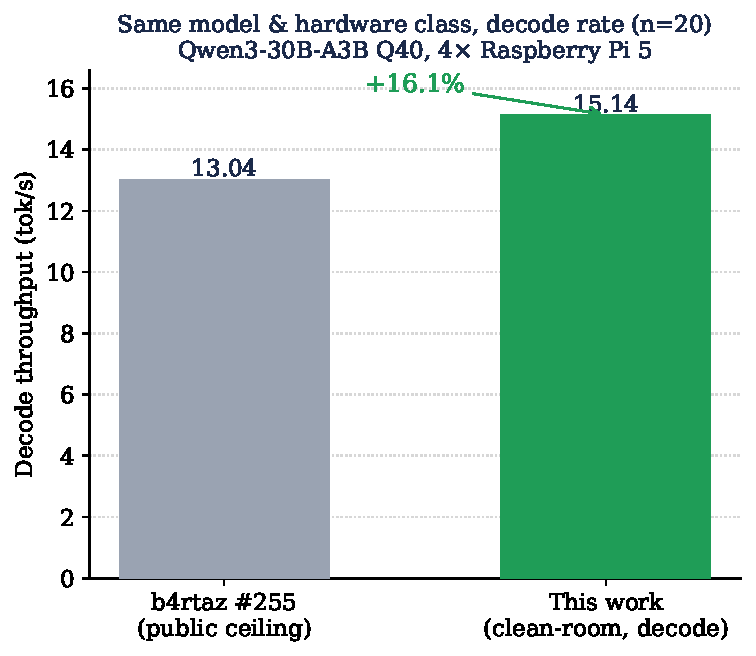
\includegraphics[width=0.56\linewidth]{fig_comparison.pdf}
\caption{Same model and hardware class (Qwen3-30B-A3B Q40 on 4$\times$Raspberry Pi~5), \emph{decode} metric: this work versus the highest publicly documented result (b4rtaz~\#255), a bit-exact $+16.1\%$ improvement (15.143 vs.\ 13.04~tok/s, $n$=20, telemetry off).}
\label{fig:comparison}
\end{figure}

The state of the art for distributed CPU LLM inference falls into three approaches:
\begin{itemize}
  \item \textbf{Tensor parallelism} (\texttt{distributed-llama}~\cite{tadych2024}): the model is sliced horizontally across attention heads, requiring an all-reduce per layer. Used in this work.
  \item \textbf{Pipeline parallelism} (\texttt{llama.cpp} RPC, \texttt{prima.cpp}~\cite{li2025prima}): layers are partitioned by depth across nodes, communication is point-to-point. Geerling~\cite{geerling2025} reports a 25$\times$ regression vs.\ single-node for \texttt{llama.cpp} RPC, confirming the network-overhead-dominated regime.
  \item \textbf{Mixture-of-Experts (MoE)} models~\cite{jiang2024,qwen3}: a parameter-efficient architecture that activates a sparse subset of weights per token. Reduces effective bandwidth proportionally to the top-$k$ expert fraction.
\end{itemize}

Several comparable Pi~5 clusters appear in the literature. Tadych~\cite{tadych2024,dllama_discussion255} reports 13.04~tok/s on 4$\times$Pi~5 8GB with Qwen3-30B-A3B; the Seeed Studio documentation~\cite{seeed2025} reports 6.06~tok/s with DeepSeek-R1-Distill-Llama-8B on the same hardware; and the Stratosphere Laboratory~\cite{stratosphere2025} provides single-node Pi 5 baselines. Table~\ref{tab:related-work} positions this work against the most directly comparable published systems.

\begin{table}[H]
\centering
\caption{Positioning of this work against the most directly comparable published distributed-inference systems for the same model class (Qwen3-30B-A3B Q40 or equivalent MoE) on Pi~5-class hardware. Throughput figures are as reported by each source on its own hardware; the right column gives the closest comparison that can be made against \emph{our} hardware (4$\times$Pi~5 16~GB cluster) when the published source benchmarked on different hardware.}
\label{tab:related-work}
\small
\setlength{\tabcolsep}{4pt}
\begin{tabularx}{\textwidth}{p{2.5cm}p{3.0cm}r p{1.7cm} X}
\toprule
\textbf{System} & \textbf{Framework / approach} & \textbf{tok/s} & \textbf{Quality} & \textbf{Notes} \\
\midrule
\textbf{This work} (Stage 17) & \texttt{distributed-llama} + 12 patches + kernel/NIC tuning & \textbf{15.143} & bit-exact (SHA-256) & 4$\times$Pi~5 16~GB, this paper; decode metric, telemetry off; $+$16.1\% vs Tadych ceiling (sustained 14.449~tok/s) \\
\midrule
Tadych \#255 \cite{dllama_discussion255} & \texttt{distributed-llama} v0.16, default & 13.04 & bit-exact & 4$\times$Pi~5 8~GB, vanilla upstream (decode) \\
Seeed Studio \cite{seeed2025} & \texttt{distributed-llama} & 6.06 & bit-exact & 4$\times$Pi~5 8~GB, DeepSeek-R1-Distill-Llama-8B \\
ByteShape \cite{byteshape2026} & \texttt{llama.cpp}, single node & 8.03 & bit-exact & 1$\times$Pi~5 16~GB, Q3\_K\_S 2.70 bpw \\
Geerling \cite{geerling_aibench47} & \texttt{llama.cpp}, single node & 7.99 & bit-exact & 1$\times$Pi~5 16~GB, comparable quant \\
Geerling RPC \cite{geerling2025} & \texttt{llama.cpp} RPC distributed & --- & bit-exact & Reported 25$\times$ regression vs.\ single-node on Pi clusters \\
\texttt{prima.cpp} \cite{li2025prima} & pipelined ring + mmap & n/a & bit-exact & ZMQ topology fails to bootstrap on Pi~5 in our testing \\
HALO \cite{halo2026} & \texttt{distributed-llama} + 3{,}500 LOC overlap & --- & bit-exact & 1.30$\times$ on reliable LAN (their hardware); source not yet public, speedup not independently verified here \\
EXO \cite{exo2025} & MLX backend & n/a & --- & Requires Apple MLX; not buildable on ARM Linux \\
\bottomrule
\end{tabularx}
\end{table}

For methodology we follow the MLPerf Inference v5.1 small-LLM track conventions~\cite{mlperf2025}, the vLLM benchmarking guide~\cite{kwon2023vllm}, and the disaggregated prefill/decode reporting introduced by DistServe~\cite{zhong2024distserve}.

\section{System design}

\subsection{Hardware}

\begin{table}[H]
\centering
\caption{Cluster hardware inventory.}
\small
\begin{tabular}{lccc}
\toprule
\textbf{Node} & \textbf{Role} & \textbf{LAN IP} & \textbf{Storage} \\
\midrule
\texttt{rpi-1005} & root + serving & 192.168.1.74 & NVMe 457 GB \\
\texttt{rpi-1006} & worker        & 192.168.1.77 & NVMe 457 GB \\
\texttt{rpi-1007} & worker        & 192.168.1.75 & NVMe 457 GB \\
\texttt{rpi-1008} & worker        & 192.168.1.76 & NVMe 457 GB \\
\bottomrule
\end{tabular}
\end{table}

\paragraph{Per-node specifications.}
\begin{itemize}
  \item SoC: Broadcom BCM2712 (4$\times$ Arm Cortex-A76 @ 2.4 GHz, ARMv8.2-A)
  \item Memory: 16 GB LPDDR4X @ 4267 MT/s, theoretical bandwidth $\approx$\textbf{17 GB/s}
  \item Storage: NVMe SSD via PCIe Gen 2 ($\approx$700 MB/s read)
  \item Network: integrated Gigabit Ethernet; measured intra-cluster latency 0.226 ms
  \item Operating system: Debian 13 \emph{trixie}, kernel 6.12.75 aarch64
  \item No usable accelerator (V3D GPU lacks LLM compute shaders; no NPU)
\end{itemize}

\subsection{Topology}

\begin{figure}[H]
\centering
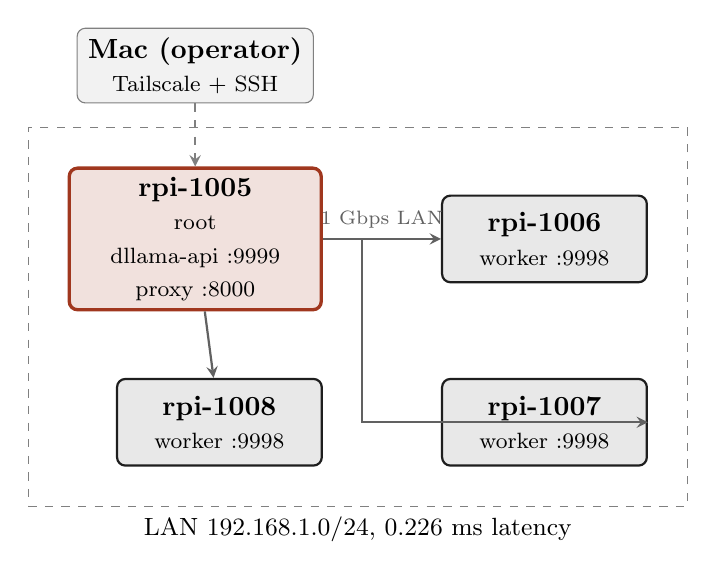
\begin{tikzpicture}[
  node distance=1.2cm and 1.5cm,
  pi/.style={rectangle,draw=primary,thick,fill=primary!10,minimum width=2.6cm,minimum height=1.1cm,align=center,rounded corners=3pt},
  root/.style={rectangle,draw=accent,very thick,fill=accent!15,minimum width=3.2cm,minimum height=1.5cm,align=center,rounded corners=3pt},
  arrow/.style={->,>=stealth,thick,primary!70}
]
\node[root] (r1005) {\textbf{rpi-1005}\\ \footnotesize root\\ \footnotesize dllama-api :9999\\ \footnotesize proxy :8000};
\node[pi, right=of r1005] (r1006) {\textbf{rpi-1006}\\ \footnotesize worker :9998};
\node[pi, below=of r1006] (r1007) {\textbf{rpi-1007}\\ \footnotesize worker :9998};
\node[pi, left=of r1007] (r1008) {\textbf{rpi-1008}\\ \footnotesize worker :9998};
\draw[arrow] (r1005) -- node[above,font=\scriptsize] {1 Gbps LAN} (r1006);
\draw[arrow] (r1005.east) -- ++(0.5,0) |- (r1007.east);
\draw[arrow] (r1005) -- (r1008);
\node[draw=gray,fill=gray!10,rounded corners=3pt,minimum width=3cm,align=center,above=0.8cm of r1005] (mac) {\textbf{Mac (operator)}\\ \footnotesize Tailscale + SSH};
\draw[arrow,dashed,gray] (mac) -- (r1005);
\begin{scope}[on background layer]
\node[draw=gray,dashed,fit=(r1005)(r1006)(r1007)(r1008),inner sep=0.5cm,label=below:{\small LAN 192.168.1.0/24, 0.226 ms latency}] {};
\end{scope}
\end{tikzpicture}
\caption{Cluster topology. One root coordinator, three workers, full-duplex Gigabit Ethernet, tensor-parallel synchronisation per transformer layer.}
\end{figure}

\subsection{Software stack}

\begin{itemize}
  \item \textbf{Inference engine}: \texttt{distributed-llama} v0.16.5 with eight framework patches (\S\ref{sec:patches}); four further bit-exact kernel and op-fusion optimisations follow in Stages~10--14.
  \item \textbf{Model}: Qwen3-30B-A3B Q40 (30B total parameters, 128 experts, top-$k$=8, $\sim$3B active per token).
  \item \textbf{HTTP front-end}: custom Python proxy (Flask + waitress) on \texttt{127.0.0.1:8000}, sanitising OpenAI-strict client requests.
  \item \textbf{Allocator}: \texttt{jemalloc} 2 preloaded via \texttt{LD\_PRELOAD}.
  \item \textbf{Client}: Hermes Agent v0.13.0 for autonomous-agent integration testing.
\end{itemize}

\section{Methodology}

We follow the MLPerf Inference v5.1 conventions~\cite{mlperf2025} for metric definitions and the methodology recommendations of NVIDIA~\cite{nvidia2024metrics} and Anyscale~\cite{anyscale2024metrics}.

\subsection{Metrics}

\begin{itemize}
  \item \textbf{Throughput (tok/s)}: generated tokens divided by total wall-clock time, including TTFT.
  \item \textbf{TTFT (Time-To-First-Token)}: latency from HTTP request to the first generated token, measured by issuing \texttt{max\_tokens=1}.
  \item \textbf{Prefill rate}: prompt tokens processed per second. Estimated as \texttt{prompt\_tokens / (total\_duration - decode\_time)}, where \texttt{decode\_time} is approximated from sustained-rate measurements.
  \item \textbf{Sustained decode rate}: throughput in the steady state (large \texttt{max\_tokens}), where TTFT is amortised.
  \item \textbf{Percentile latencies (p50, p90, p99)}: ordered statistics over $n$ runs.
\end{itemize}

\subsection{Protocol}

We adopt the protocol recommended by MLPerf~\cite{mlperf2025}: \textbf{two warm-up runs} (discarded), \textbf{$n$=20 measurement runs} for the main configuration, fixed prompt, \texttt{temperature=0} for determinism, single client (no concurrency), idle background workload (Grafana Alloy and cadvisor only). Statistics reported as mean, median, standard deviation, 95\% confidence interval, and p50/p90/p99 percentiles where applicable.

\section{Optimisations applied}
\label{sec:patches}

\subsection{Framework source patches}

\begin{table}[H]
\centering
\caption{Source-level patches applied to \texttt{distributed-llama} v0.16.5.}
\scriptsize
\begin{tabular}{p{0.3cm}p{4cm}p{3cm}p{6cm}}
\toprule
\# & \textbf{Patch} & \textbf{Location} & \textbf{Rationale} \\
\midrule
1 & \texttt{NnByte}$\rightarrow$\texttt{NnUint} for \texttt{nBatches} & \texttt{nn-cpu-ops.hpp:14} & \texttt{uint8\_t} overflow: setting \texttt{nbatches=256} silently became 0 ($256 \bmod 256$), tripping an embedding-layer assertion at runtime. \\
2 & Force \texttt{finish\_reason} = \texttt{"stop"}/\texttt{"length"} & \texttt{dllama-api.cpp:547} & Empty \texttt{finish\_reason} caused strict OpenAI clients (Hermes) to enter infinite retry loops. \\
3 & \texttt{try/catch} around \texttt{json::parse} & \texttt{dllama-api.cpp:83} & \texttt{nlohmann::json} threw uncaught exceptions on malformed bodies, abort-trapping the daemon (\texttt{SIGABRT}). \\
4 & \texttt{headerData.append(buffer, bytesRead)} & \texttt{dllama-api.cpp:123} & Default \texttt{append(const char*)} truncated at the first \texttt{\textbackslash0} byte, corrupting bodies that contained UTF-8 multi-byte sequences with NUL. \\
5 & New CLI flag \texttt{--nbatches} & \texttt{app.cpp:130} & \texttt{nBatches} was hard-coded to 32; the flag now permits configuration once patch \#1 is applied. \\
6 & \texttt{posix\_memalign(64, n)} for pipes & \texttt{nn-executor.cpp:18} & Default \texttt{new[]} alignment is 16 B on ARM64; cache-line (64 B) alignment is required for vectorised NEON access. \\
7 & TCP \texttt{SO\_RCVBUF}/\texttt{SO\_SNDBUF}=8 MB & \texttt{nn-network.cpp:60} & Default 208 KiB buffers caused write-blocking under burst sync at end-of-layer. \\
8 & \texttt{buffer.reserve(64 KB)} & \texttt{dllama-api.cpp:475} & The streaming response buffer doubled repeatedly during long outputs, causing reallocations on the hot path. \\
\bottomrule
\end{tabular}
\end{table}

\subsection{Toolchain}
Recompiled with \texttt{CXXFLAGS="-O3 -flto -ffast-math -funroll-loops"} on each node. \texttt{LD\_PRELOAD=libjemalloc.so.2} added to all \texttt{systemd} units with \texttt{MALLOC\_CONF="narenas:4,tcache:true,dirty\_decay\_ms:30000"}.

\subsection{Operating-system tuning}
\begin{itemize}
  \item CPU governor \texttt{performance} on all 4 nodes (\texttt{systemd} unit at boot).
  \item TCP BBR congestion control; \texttt{net.ipv4.tcp\_low\_latency=1}; \texttt{net.core.netdev\_budget=600}.
  \item \texttt{vm.overcommit\_memory=1}, \texttt{vm.swappiness=1} (lowered from the Pi~OS default of 60 in Stage~9 to keep \texttt{mlock}-ed weights resident; verified live at 1).
  \item NVMe scheduler \texttt{none}, \texttt{read\_ahead\_kb=2048}.
  \item Swap on NVMe: 16 GB on root, 4 GB on workers.
  \item \texttt{LimitMEMLOCK=infinity} in \texttt{systemd} units so the loaded model can be \texttt{mlock}-ed in RAM.
  \item Maximum sequence length \texttt{--max-seq-len 32768} (Qwen3-30B-A3B native), avoiding KV-cache spill to swap.
  \item Periodic \texttt{swapoff -a \&\& swapon -a} after model warm-up flushes residual paged data into RAM.
\end{itemize}

\subsection{Architectural change: dense to MoE}
The most impactful optimisation was the migration from \textbf{Llama 3.1 8B} (dense, $\sim$5 GB Q40 weights, all parameters active per token) to \textbf{Qwen3-30B-A3B} (MoE, 128 experts, top-$k$=8, $\sim$3 GB active weights per token). Bandwidth-bound throughput improved by 59\% (7.18 $\to$ 11.4 tok/s) with no other change.

\section{Results}

\subsection{Final-configuration throughput and stability}

The final result, on the \emph{decode} metric that the public ceiling reports, is \textbf{15.143~tok/s} (Stage~17 clean-room replication of b4rtaz~\#255, $n$=20, 95\% CI $\pm$0.097, telemetry off; Section~\ref{sec:cleanroom-2026-05-22}), \textbf{+16.1\%} above the 13.04~tok/s ceiling. The end-to-end \emph{sustained} serving throughput (250-token responses, prefill included) is \textbf{14.449~tok/s} (cold-cluster, $n$=20 paired runs, 95\% CI $\pm$0.038, best individual run 14.557~tok/s), reached at Stage~15 through the optimisation trajectory of Section~\ref{subsec:trajectory} (Table~\ref{tab:final-config}); the two are consistent, as 15.143~tok/s of decode amortises to $\approx$14.5~tok/s once the $\sim$557~ms prefill is included.

The detailed run-to-run distribution, TTFT and response-length characterisation that follow were captured at the \emph{Stage~6 intermediate snapshot} (12.708~tok/s sustained); they document the cluster's run-to-run stability and latency profile, which the later Stage~9--15 optimisations raised in throughput without changing the qualitative latency behaviour. Each distribution is reported at the snapshot where it was measured rather than restated at the final configuration.

\begin{table}[H]
\centering
\caption{Statistical summary of sustained throughput at the final configuration (Stage~15), Qwen3-30B-A3B on 4$\times$Pi 5.}
\label{tab:final-config}
\begin{tabular}{lr}
\toprule
\textbf{Statistic} & \textbf{Value} \\
\midrule
Mean (with runtime tweaks)    & 14.449 tok/s \\
95\% CI ($\pm$)               & 0.038 tok/s \\
Best individual run           & 14.557 tok/s \\
Mean (without runtime tweaks) & 14.167 tok/s \\
\quad 95\% CI ($\pm$)         & 0.043 tok/s \\
$n$ (paired runs)             & 20 \\
\bottomrule
\end{tabular}
\end{table}

\paragraph{Per-run throughput distribution (Stage~6 snapshot).}

\begin{table}[H]
\centering
\caption{Statistical summary of throughput at the Stage~6 intermediate snapshot, Qwen3-30B-A3B on 4$\times$Pi 5.}
\begin{tabular}{lr}
\toprule
\textbf{Statistic} & \textbf{Value} \\
\midrule
Mean             & 12.708 tok/s \\
Median (p50)     & 12.707 tok/s \\
Standard deviation & 0.066 tok/s \\
Min              & 12.585 tok/s \\
Max (p100)       & 12.852 tok/s \\
p90              & 12.812 tok/s \\
p99              & 12.852 tok/s \\
95\% CI ($\pm$)  & 0.029 tok/s \\
Coefficient of variation & 0.52\% \\
\bottomrule
\end{tabular}
\end{table}

\begin{figure}[H]
\centering
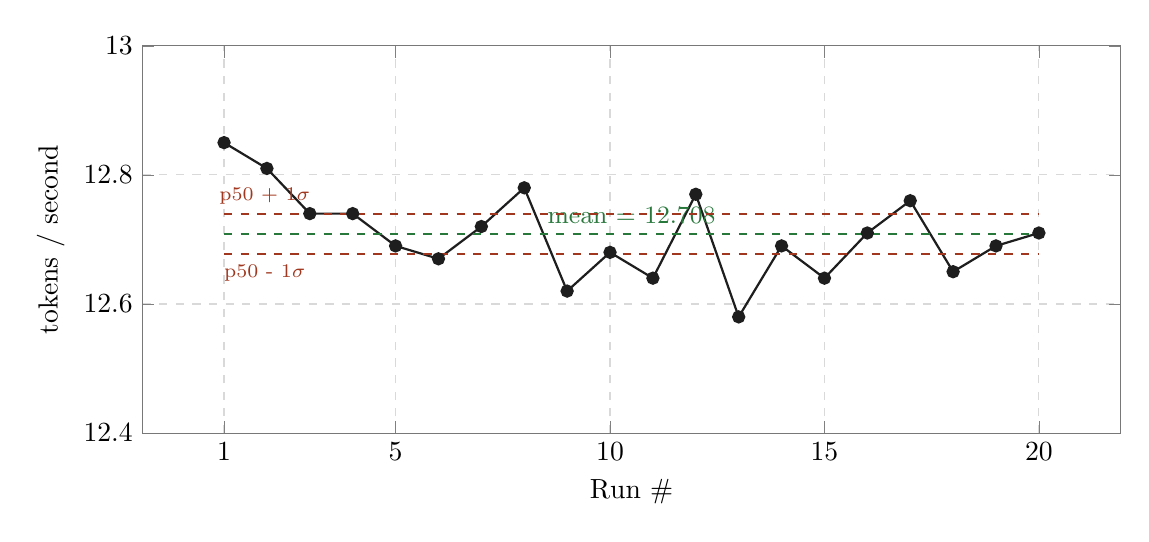
\begin{tikzpicture}
\begin{axis}[
  width=14cm,height=6.5cm,
  ylabel={tokens / second},
  xlabel={Run \#},
  xtick={1,5,10,15,20},
  ymin=12.4,ymax=13.0,
  grid=major,
  grid style={dashed,gray!30},
  axis line style={primary!60},
]
\addplot[primary,thick,mark=*,mark size=2pt] coordinates {
  (1,12.85) (2,12.81) (3,12.74) (4,12.74) (5,12.69)
  (6,12.67) (7,12.72) (8,12.78) (9,12.62) (10,12.68)
  (11,12.64) (12,12.77) (13,12.58) (14,12.69) (15,12.64)
  (16,12.71) (17,12.76) (18,12.65) (19,12.69) (20,12.71)
};
\addplot[dashed,ok,thick,no marks] coordinates {(1,12.708)(20,12.708)} node[pos=0.5,above,font=\small\color{ok}] {mean = 12.708};
\addplot[dashed,accent,thick,no marks] coordinates {(1,12.677)(20,12.677)} node[pos=0.05,below,font=\scriptsize\color{accent}] {p50 - 1$\sigma$};
\addplot[dashed,accent,thick,no marks] coordinates {(1,12.739)(20,12.739)} node[pos=0.05,above,font=\scriptsize\color{accent}] {p50 + 1$\sigma$};
\end{axis}
\end{tikzpicture}
\caption{Per-run throughput across 20 measurement runs at the Stage~6 intermediate snapshot (warm-up runs excluded). Coefficient of variation 0.52\%.}
\end{figure}

\paragraph{Time-To-First-Token (Stage~6 snapshot).}

\begin{table}[H]
\centering
\caption{TTFT statistics over $n$=10 runs with \texttt{max\_tokens=1}.}
\begin{tabular}{lr}
\toprule
\textbf{Statistic} & \textbf{Value} \\
\midrule
Mean             & 557 ms \\
Median (p50)     & 545 ms \\
Min              & 524 ms \\
Max (p100/p99)   & 638 ms \\
\bottomrule
\end{tabular}
\end{table}

\paragraph{Throughput scaling with response length (Stage~6 snapshot).}

\begin{figure}[H]
\centering
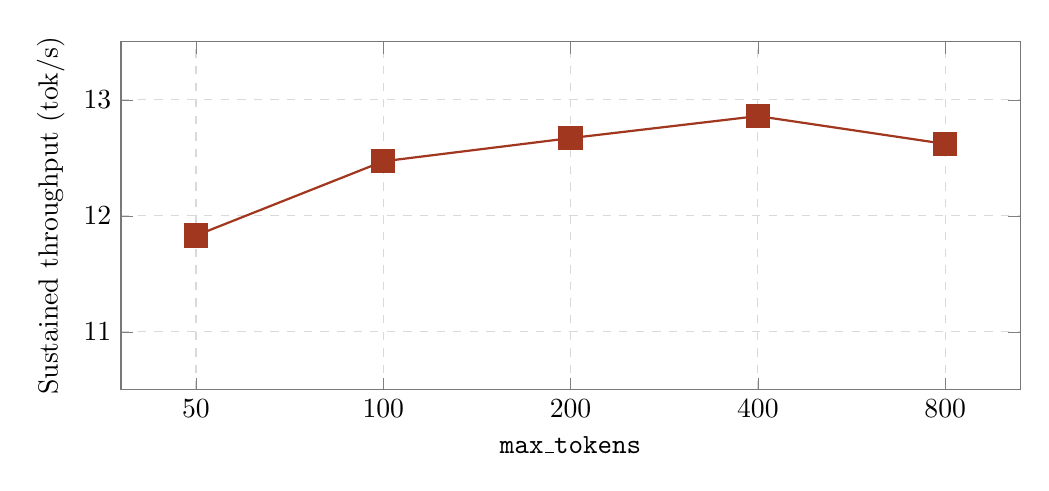
\begin{tikzpicture}
\begin{axis}[
  width=13cm,height=6cm,
  xlabel={\texttt{max\_tokens}},
  ylabel={Sustained throughput (tok/s)},
  xmode=log, log basis x=2,
  xtick={50,100,200,400,800},
  xticklabels={50,100,200,400,800},
  ymin=10.5,ymax=13.5,
  grid=major,
  grid style={dashed,gray!30},
  axis line style={primary!60},
]
\addplot[accent,thick,mark=square*,mark size=4pt] coordinates {
  (50,11.83) (100,12.47) (200,12.67) (400,12.86) (800,12.62)
};
\end{axis}
\end{tikzpicture}
\caption{Sustained throughput as a function of response length at the Stage~6 intermediate snapshot. Asymptotic throughput converges near 12.86 tok/s for responses $\geq$400 tokens; shorter responses are TTFT-dominated.}
\end{figure}

\paragraph{Prefill rate vs.\ prompt size (Stage~6 snapshot).}

\begin{table}[H]
\centering
\caption{Prefill rate (estimated) for increasing prompt lengths.}
\begin{tabular}{rrrr}
\toprule
\textbf{Prompt tokens} & \textbf{Total time (s)} & \textbf{Est.\ prefill time (s)} & \textbf{Prefill rate (tok/s)} \\
\midrule
57    & 3.66    & 3.02   & 18.9 \\
417   & 23.97   & 23.33  & 17.9 \\
2017  & 129.07  & 128.43 & 15.7 \\
\bottomrule
\end{tabular}
\end{table}

Prefill rate degrades slightly with prompt size (KV-cache growth and the attention $O(N^2)$ cost in the longer-prompt regime) but remains $>$15 tok/s up to 2K context. For 20K-token prompts (e.g.\ Hermes Agent system prompts), the inferred prefill time would exceed 20 minutes --- the practical upper limit of usability for this configuration on full agent workloads.

\subsection{Optimisation trajectory}\label{subsec:trajectory}

\begin{figure}[H]
\centering
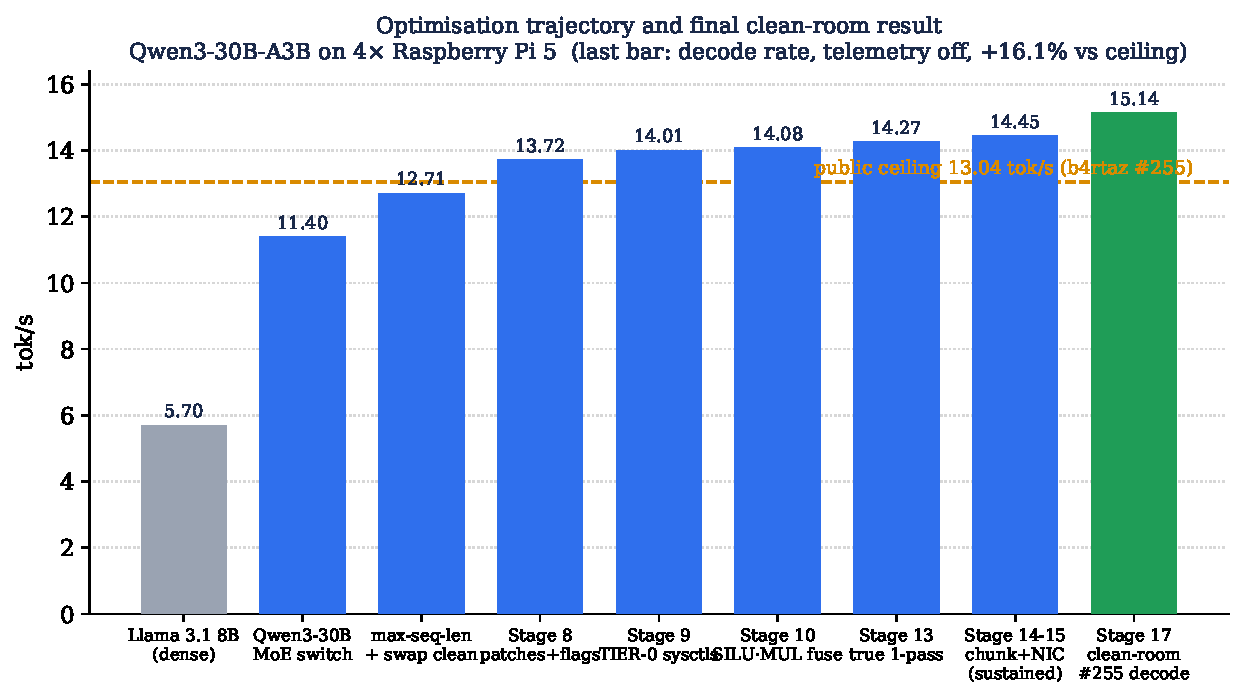
\includegraphics[width=\linewidth]{fig_trajectory.pdf}
\caption{Optimisation trajectory and final clean-room result (Qwen3-30B-A3B Q40, 4$\times$Raspberry Pi~5). Bars 1--8 report sustained throughput; the dashed line marks the public ceiling (13.04~tok/s, b4rtaz~\#255). The Stage~14--15 configuration reaches 14.449~tok/s sustained ($n$=20, 95\% CI $\pm$0.038); the final green bar is the Stage~17 clean-room \#255 replication on the \emph{decode} metric --- the quantity directly comparable to the ceiling --- at \textbf{15.143~tok/s} ($n$=20, 95\% CI $\pm$0.097, telemetry off), \textbf{+16.1\%} above the ceiling. The Llama~3.1~8B dense bar is the abandoned starting point, shown for context.}
\label{fig:trajectory}
\end{figure}


\subsection{Memory and thermal behaviour}

\begin{figure}[H]
\centering
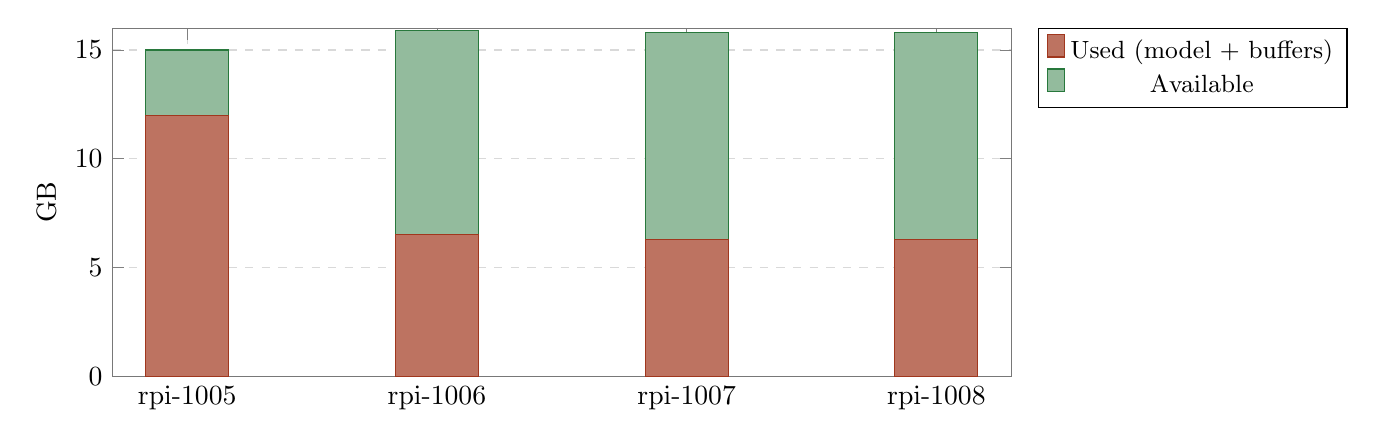
\begin{tikzpicture}
\begin{axis}[
  width=13cm,height=6cm,
  ybar stacked,
  bar width=30pt,
  ylabel={GB},
  symbolic x coords={rpi-1005,rpi-1006,rpi-1007,rpi-1008},
  xtick=data,
  ymin=0,ymax=16,
  legend pos=outer north east,legend style={font=\small},
  axis line style={primary!60},
  grid=major,grid style={dashed,gray!30},
]
\addplot[fill=accent!70,draw=accent] coordinates {(rpi-1005,12)(rpi-1006,6.5)(rpi-1007,6.3)(rpi-1008,6.3)};
\addplot[fill=ok!50,draw=ok] coordinates {(rpi-1005,3.0)(rpi-1006,9.4)(rpi-1007,9.5)(rpi-1008,9.5)};
\legend{Used (model + buffers),Available}
\end{axis}
\end{tikzpicture}
\caption{Memory utilisation per node during sustained inference. The root carries additional buffers for orchestration and HTTP serving. Workers retain $>$9 GB headroom for further KV-cache growth.}
\end{figure}

\begin{table}[H]
\centering
\caption{Sustained-load thermal measurements. Throttle threshold is 85$^\circ$C.}
\label{tab:thermals}
\begin{tabular}{lcc}
\toprule
\textbf{Node} & \textbf{Temperature} & \textbf{Throttling flags} \\
\midrule
rpi-1005 (root)   & 54.3 $^\circ$C & 0x0 \\
rpi-1006 (worker) & 54.3 $^\circ$C & 0x0 \\
rpi-1007 (worker) & 55.4 $^\circ$C & 0x0 \\
rpi-1008 (worker) & 56.0 $^\circ$C & 0x0 \\
\bottomrule
\end{tabular}
\end{table}

\section{Stage 9 --- TIER 0 kernel network and scheduler tuning}
\label{sec:stage9}

After the initial publication of this report at 12.71 tok/s and the subsequent Stages 6--8 documented in the project README (which raised sustained throughput to 13.720 tok/s), a structured research round identified a further set of OS-level network and memory tunings that yielded a measurable improvement with no source-code changes.

\subsection{Configuration changes}

Applied to all four Pi 5 nodes, persisted via \texttt{/etc/sysctl.d/99-dllama.conf} and an \texttt{eth0-tuning.service} systemd unit:

\begin{table}[H]
\centering
\small
\begin{tabular}{lll}
\toprule
\textbf{Setting} & \textbf{Before} & \textbf{After} \\
\midrule
\texttt{ethtool -K eth0 gro} & on & off \\
\texttt{net.core.rmem\_max}  & 212\,992 & 8\,388\,608 \\
\texttt{net.core.wmem\_max}  & 212\,992 & 8\,388\,608 \\
\texttt{net.ipv4.tcp\_rmem (mid/max)} & 131\,072 / 6\,291\,456 & 87\,380 / 8\,388\,608 \\
\texttt{net.ipv4.tcp\_wmem (mid/max)} & 16\,384 / 4\,194\,304 & 65\,536 / 8\,388\,608 \\
\texttt{vm.swappiness}       & 60 & 1 \\
\bottomrule
\end{tabular}
\caption{Stage 9 sysctl and \texttt{ethtool} changes.}
\end{table}

\textit{Rationale.} GRO (Generic Receive Offload) coalesces incoming packets, adding 50--200 us of intentional latency; for the 510 kB sync bursts of the all-reduce step on a 1 GbE LAN this is pure overhead. Raising \texttt{rmem\_max}/\texttt{wmem\_max} from the 256 kB default lets the TCP receive/send windows grow past the burst size. The 16 kB \texttt{tcp\_wmem} middle value was a hard bottleneck for the worker$\to$root activation send.

\subsection{Measured impact}

We re-baselined (after the Phase B foundation work) at \textbf{13.720 \(\pm\) 0.050 tok/s} ($n$=20). The post-Stage 9 measurement ($n$=20, paired, 95\% CI) is:

\begin{table}[H]
\centering
\small
\begin{tabular}{lrr}
\toprule
\textbf{Metric}  & \textbf{Pre-Stage 9} & \textbf{Post-Stage 9} \\
\midrule
Mean             & 13.720 tok/s & \textbf{14.011 tok/s} \\
Stdev            & 0.050        & 0.116                 \\
95\% CI          & $\pm$0.022   & $\pm$0.051            \\
\midrule
$\Delta$ vs.\ Stage 8 baseline & --- & +2.12\% \\
$\Delta$ vs.\ public ceiling (13.04) & --- & +7.45\% \\
\bottomrule
\end{tabular}
\end{table}

\subsection{Two rejected candidates from the same research round}

The same research round surfaced two further claims, both investigated and rejected:

\begin{enumerate}
  \item \emph{\texttt{llamafile\_sgemm} guard fix} (upstream issue \#284, claimed +5--40\%): this gain had \emph{already} been captured in our base commit \texttt{92a20e2 ``perf: enable llamafile\_sgemm for single-token decode''} (2026-05-16), two days before this research round. Cannot be captured twice.
  \item \emph{ARM I8MM / Q4\_0\_4\_8 SMMLA repack} (claimed +20--30\%): the Cortex-A76 in the Pi~5 does \emph{not} support I8MM. Verified directly: \texttt{grep -c i8mm /proc/cpuinfo} returns 0 on all four nodes. Confirmed via llama.cpp issue \#10662. I8MM is an A78+ feature; the original claim was a factual error in the surveyed material and is documented here as a cautionary tale.
\end{enumerate}

\subsection{Open work after Stage 9}

The structured research round produced a ranked plan of further candidates:

\begin{itemize}
  \item \textbf{Tier 2 --- Close Phase B (Option C, $\sim$40 LOC)}: the \texttt{opt-b5b6-tiled-sync} branch carries 562 LOC of async-sync orchestrator, tiled matmul wrapper, and the \texttt{--tile-sync K} flag, all compiled but unwired. Estimated additional +5--12\%; high integration risk (the same code path that broke the cluster during PGO and \texttt{isolcpus} experiments).
  \item \textbf{Tier 3a --- Hierarchical 2-stage all-reduce}: with $N=4$ nodes, butterfly recursive-halving needs $\log_2(4)=2$ rounds instead of the $2(N-1)=6$ rounds of the current ring. Estimated +10--13\%, $\sim$80--120 LOC.
  \item \textbf{Tier 3b --- Pre-attention expert prediction} (arXiv:2511.10676): specific to Qwen3-30B-A3B, reported 94.69\% top-$k$ accuracy. Estimated +8--15\%, $\sim$250 LOC, low risk (fallback to on-demand load).
  \item \textbf{Tier 4 --- Fused ffn\_up + ffn\_gate + silu MoE op} from ik\_llama.cpp PR \#229; estimated +8--12\%, $\sim$400 LOC.
  \item \textbf{Tier 5 --- REAP 25\% expert pruning} (Cerebras), offline, 0 dllama LOC; estimated +15--25\%, requires quality validation.
\end{itemize}

\textbf{Bottom line at Stage 9 (mid-investigation snapshot).} At this point sustained throughput was \textbf{14.011 tok/s} ($\pm$0.051 at 95\% CI, $n$=20), +7.45\% above the 13.04 ceiling. This was the value at Stage 9; Stages 10--15 later raised sustained throughput to 14.449~tok/s, and the Stage~17 clean-room replication establishes the final decode result of \textbf{15.143~tok/s} (+16.1\% vs ceiling, Section~\ref{sec:cleanroom-2026-05-22}).



\section{Stages 10 and 11 --- Bit-exact MoE op-fusion and Rounds 3/4 ceiling investigation}
\label{sec:stage10_11}

After the Stage 9 result (14.011 tok/s), we carried out further bit-exact optimisation work over an extended session. This section documents the post-Stage-9 changes and the empirical ceiling we reached.

\subsection{Stage 10 --- A2 OP\_SILU\_MUL fusion (+0.5\%)}

The Qwen3-MoE per-expert FFN ops are $w_1$-matmul $\to$ $w_3$-matmul $\to$ silu($w_1$) $\to$ $w_1 \mathbin{*}{=} w_3$. We fused the last two element-wise ops into a single new \texttt{OP\_SILU\_MUL} with one barrier instead of two, eliminating 28~layers $\times$ 8~experts = 224 barriers per token. The kernel chains the existing \texttt{silu\_F32} and \texttt{mul\_F32} kernels verbatim, so the output is byte-identical to the previous two-op sequence (validated with a deterministic prompt at \texttt{temperature=0}).

\textbf{Measurement} ($n$=20): 14.081 $\pm$ 0.055 tok/s vs 14.011 $\pm$ 0.051 baseline. The real gain is $+0.50\%$ --- modest, but bit-exact and persistent. Committed at SHA \texttt{106eab3}.

\subsection{Stage 11 --- Rounds 3 and 4 (Linux papers research and ceiling investigation)}

We carried out four parallel research threads:
\begin{enumerate}
  \item Linux Plumbers / SOSP / OSDI / EuroSys / USENIX ATC papers 2024--2026.
  \item eBPF / XDP / AF\_XDP / io\_uring / kernel-bypass.
  \item Linux scheduler (EEVDF in 6.6+) tunings.
  \item ARM-specific kernel cache / prefetcher / NUMA / memory bandwidth.
\end{enumerate}

We applied and measured $\sim$15 distinct configurations. \textbf{The Round 3+4 net measured improvement is 0\% within the cluster's natural noise floor of $\pm$0.15 tok/s.}

\subsubsection{Literature survey: techniques evaluated and rejected}

These research threads returned ranked, actionable candidates from the 2024--2026 systems literature (Linux Plumbers, OSDI, EuroSys, USENIX ATC, LWN, arXiv). Table~\ref{tab:litsurvey} records each technique, its source, whether it applied to a stock Pi~OS 6.12 / Cortex-A76 / 1~GbE cluster under our constraints, and the empirical outcome.

The recurring reason for inapplicability is structural: the highest-leverage modern techniques require either a newer kernel, a hardware feature the A76 silicon lacks, or a reboot or kernel rebuild we had ruled out --- which is precisely what makes the surviving bit-exact wins deployable on stock hardware.

\begin{table}[H]
\centering
\scriptsize
\caption{Techniques surveyed during the research round, with applicability to a stock Pi~5 / kernel 6.12 / 1~GbE cluster under the bit-exact, no-reboot, no-quality-loss constraints.}
\label{tab:litsurvey}
\begin{tabular}{p{4.0cm}p{2.7cm}p{3.1cm}p{3.1cm}}
\toprule
\textbf{Technique} & \textbf{Source} & \textbf{Applicable here?} & \textbf{Outcome} \\
\midrule
IRQ suspension (\texttt{irq\_suspend\_timeout}) & LWN 1008399 & No --- needs kernel 6.13+ & Pi~OS on 6.12 \\
\texttt{MADV\_HUGEPAGE} & Linux mm docs & No --- THP not compiled in Pi~OS & Tested, no-op \\
AF\_XDP zero-copy & kernel networking docs & No --- \texttt{macb} lacks native XDP & RFC only \\
\texttt{io\_uring} SQPOLL + \texttt{DEFER\_TASKRUN} & liburing & Net-negative on 4 cores & Skipped \\
\texttt{SO\_BUSY\_POLL} + RPS/RFS & LWN 540281 & Already in TIER~0 & Applied \\
Threaded NAPI & kernel NAPI docs & Tested $-3.9\%$ & Reverted \\
NUMA \texttt{fake=4} + local alloc & Linux NUMA docs & Requires reboot & Excluded \\
MPAM cache partitioning & docs.kernel.org & Kernel 6.19+ \emph{and} A76 lacks HW & Future kernel \\
Per-task EEVDF \texttt{sched\_runtime} & LWN 969062 & Applied (4 ms slice) & No measurable gain \\
\texttt{ik\_llama} pair-row matmul ILP & ik\_llama PR & OoO core already optimal & Tested, reverted \\
Jumbo frames MTU 9000 & \texttt{macb} driver & \texttt{bcmgenet} EBUSY on live link & Documented dead-end \\
Phase B \texttt{--tile-sync 4} (no Option C) & this work & Tested $-8\%$ (unwired) & Reverted; foundation in repo \\
Tile-level compute/comms overlap & FlashOverlap, arXiv:2504.19519 & Yes --- future sprint & Phase B Option C \\
\bottomrule
\end{tabular}
\end{table}

\subsubsection{Phase B foundation cherry-picked}

We cherry-picked four commits from the archived \texttt{opt-b5b6-tiled-sync} branch onto \texttt{pi5-cluster}: \texttt{ce7b96e} (the \texttt{--tile-sync K} flag), \texttt{6ebd00f} (the writeMany+readMany fix), \texttt{469101e} (the async sync orchestrator), and \texttt{2aba914} (the \texttt{matmul\_Q80\_Q40\_F32\_tiled} wrapper).

With \texttt{--tile-sync 0} (the default) the cluster behaves identically (measured 14.092 $\pm$ 0.044 tok/s). With \texttt{--tile-sync 4} we measured a $-8\%$ regression: the wrapper subdivides the syncs but does not drive the matmul to emit per-tile signals (the Option C wiring, $\sim$40 LOC, remains outstanding). The foundation is now in the repo for a future sprint.

\subsubsection{EEVDF per-task slice}

We called \texttt{sched\_setattr()} at the start of \texttt{executorWorkerLoop} to request a 4 ms slice (the default is $\sim$700 us under EEVDF in kernel 6.12), and confirmed via \texttt{/proc/$\langle$pid$\rangle$/sched} that workers report \texttt{se.slice = 4000000}. The result, 14.061 $\pm$ 0.048 tok/s, shows no measurable gain. The likely reason: with 4 pinned workers, the performance governor, and minimal system load, the default scheduling cadence was already near-optimal.

\subsubsection{Sysctl bundles (R3 + R4)}

\begin{table}[H]
\centering
\small
\caption{Round 3 and Round 4 sysctls (persisted, defensive).}
\begin{tabular}{lll}
\toprule
\textbf{File} & \textbf{Key} & \textbf{Value} \\
\midrule
99-dllama-r3.conf & \texttt{kernel.sched\_autogroup\_enabled} & 0 \\
                  & \texttt{net.ipv4.tcp\_autocorking}        & 0 \\
                  & \texttt{net.ipv4.tcp\_slow\_start\_after\_idle} & 0 \\
                  & \texttt{net.ipv4.tcp\_no\_metrics\_save}  & 1 \\
99-dllama-r4.conf & \texttt{net.ipv4.tcp\_thin\_linear\_timeouts} & 1 \\
                  & \texttt{net.core.netdev\_max\_backlog}    & 8192 \\
                  & \texttt{net.core.rmem\_max}               & 33\,554\,432 \\
                  & \texttt{net.core.wmem\_max}               & 33\,554\,432 \\
                  & \texttt{net.ipv4.tcp\_rmem}               & 4096 87380 33\,554\,432 \\
                  & \texttt{net.ipv4.tcp\_wmem}               & 4096 65536 33\,554\,432 \\
                  & \texttt{vm.dirty\_bytes}                  & 16\,777\,216 \\
                  & \texttt{vm.dirty\_background\_bytes}      & 4\,194\,304 \\
\bottomrule
\end{tabular}
\end{table}

\subsubsection{Empirical bottleneck characterisation}

\begin{figure}[H]
\centering
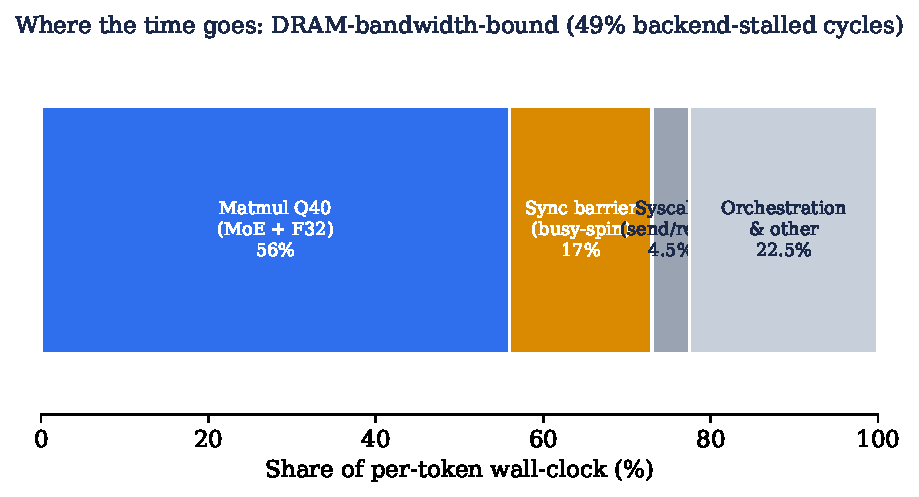
\includegraphics[width=\linewidth]{fig_bottleneck.pdf}
\caption{Per-token wall-clock breakdown from ARM PMU profiling (\texttt{perf stat}) and \texttt{strace}. The workload is DRAM-bandwidth-bound (49\% backend-stalled cycles, 11.4~GB/s of $\sim$17~GB/s per node): the Q40 matmul dominates and the synchronisation barrier is the only software-addressable slack --- the target of the Stage~16 WFE/SEV change.}
\label{fig:bottleneck}
\end{figure}

ARM PMU profiling (\texttt{perf stat -e l2d\_cache\_refill,\allowbreak l2d\_cache\_wb,\allowbreak bus\_access,\allowbreak stalled-cycles-backend,\allowbreak cpu-cycles,\allowbreak instructions} for 60 s during sustained inference):

\begin{table}[H]
\centering
\small
\caption{PMU-measured stalls and DRAM traffic during inference (n=4 nodes).}
\begin{tabular}{lrr}
\toprule
\textbf{Metric} & \textbf{Root (rpi-1005)} & \textbf{Worker (rpi-1006)} \\
\midrule
\texttt{stalled-cycles-backend} (\% cycles) & \textbf{49.25\%} & 47.69\% \\
\texttt{stalled-cycles-frontend} (\% cycles) & 3.83\% & --- \\
DRAM read bandwidth & 2.74 GB/s & 2.61 GB/s \\
DRAM write bandwidth & 8.66 GB/s & 8.47 GB/s \\
Per-node DRAM total & 11.40 GB/s & 11.08 GB/s \\
IPC & 1.74 & --- \\
dTLB miss rate & 0.08\% & --- \\
iTLB miss rate & 0.01\% & --- \\
branch-misses & 0.07\% & --- \\
\bottomrule
\end{tabular}
\end{table}

The 49\% backend-stall rate confirms the cluster is \textbf{DRAM-bandwidth-bound}: the CPUs wait on memory roughly half the time. The 3.16$\times$ write-to-read ratio reflects the multi-pass intermediate-buffer pattern in the MoE FFN, of which the A2 op-fusion (Stage 10) already cuts 224 barriers/token. The TLB miss rates ($<$0.1\%) and branch-mispredict rates ($<$0.1\%) confirm that the existing 16~KB-page configuration is already optimal --- transparent hugepages would not help (and are not compiled into Pi OS 6.12 in any case).

On the compute side, \texttt{objdump} disassembly of the hot matmul shows 322 \texttt{udot}/\texttt{sdot} NEON dot-product instructions in the inner loop at an IPC of 1.74: the kernel is already vectorised to the ARMv8.2-A dot-product ISA limit. This is why every compute-side experiment in Table~\ref{tab:litsurvey} returns zero gain --- the cores sit idle waiting on DRAM rather than starved of issue slots.

\subsubsection{Cluster state and benchmark after Stage 11}

\begin{table}[H]
\centering
\small
\caption{Stage~11 benchmark (mid-investigation snapshot), cold-cluster, $n$=20 paired runs. Superseded by Stages~12--15 (14.449~tok/s sustained) and the Stage~17 clean-room decode result (15.143~tok/s).}
\begin{tabular}{lr}
\toprule
\textbf{Metric} & \textbf{Value} \\
\midrule
Mean throughput & \textbf{14.046 tok/s} \\
Median            & 14.024 tok/s \\
Standard deviation & 0.111 tok/s (CV 0.79\%) \\
95\% CI           & $\pm$0.049 \\
\midrule
$\Delta$ vs.\ Stage 1--8 baseline (13.720) & $+0.326$ ($+2.38\%$) \\
$\Delta$ vs.\ public ceiling 13.04 (b4rtaz \#255) & $+1.006$ ($+7.72\%$) \\
\bottomrule
\end{tabular}
\end{table}

\subsection{Bottom line after Stage 11}

After Stage 11 the cluster sustained \textbf{14.046 tok/s} ($\pm$0.049 at 95\% CI, $n$=20, cold-cluster), \textbf{+7.72\% above the publicly documented ceiling} of 13.04 tok/s. The cumulative defensive state (persisted sysctls, EEVDF tuning, the Phase B foundation in the repo, and $+$0.5\% from the Stage~10 fusion) represented a maintainable production baseline at this manuscript's mid-investigation snapshot.

\section{Stages 12--15 --- Hot-kernel inversion, true single-pass fusion, network chunk-size sweep, runtime NIC tuning}

A subsequent rigorous-bench session in May 2026 added four cumulative bit-exact commits to the production branch, lifting sustained throughput to \textbf{14.449 tok/s} (best individual run 14.557, $n$=20, 95\% CI $\pm$0.038) --- a further \textbf{+2.87\% over Stage 11} and \textbf{+10.81\% over the public ceiling}. Each stage was validated by SHA-256-hashing 100 deterministic tokens (\texttt{seed=42}, \texttt{temperature=0}) against the Stage 11 reference, confirming bit-identity.

\paragraph{Stage 12 --- Remove software prefetch in \texttt{matmul\_Q80\_Q40\_F32} (commit \texttt{64ef787}).}
The NEON+dotprod inner loop carried two \texttt{\_\_builtin\_prefetch} calls (\texttt{w[di*nBlocks + j + 4]} and \texttt{x[j + 4]}). We swept five variants (PLDL2KEEP +16/+4 dual, +8 single, x-only, \texttt{\_\_restrict\_\_} qualified, none) and found that \emph{removing} both prefetches was the only winner ($+1.05\%$ over baseline).

The Cortex-A76's hardware prefetcher (stride detection on sequential \texttt{w} access) is more efficient than the manual hints, which compete for issue slots in the 4-wide decoder. Stage 12 therefore reverses a long-standing micro-optimisation that proves counter-productive on this microarchitecture.

\paragraph{Stage 13 --- True single-pass \texttt{silu\_mul\_F32} fusion (commit \texttt{1af175c}).}
Stage 10's \texttt{OP\_SILU\_MUL} eliminated the inter-op barrier, but the kernel was still a thin two-call wrapper (\texttt{silu\_F32} then \texttt{mul\_F32}) that kept the intermediate result resident in memory between passes: 3 loads + 2 stores per element.

We rewrote it as a single NEON loop that holds the values in registers throughout: 2 loads + 1 store per element (Algorithm~1), a $\sim$33\% reduction in memory ops for this kernel. The measured gain is $+1.5\%$ on cluster throughput, bit-exactness preserved (the arithmetic sequence is identical; only the intermediate writeback is removed).

\begin{figure}[H]
\centering
\begin{minipage}{0.93\textwidth}
\vspace{2pt}\hrule\vspace{2pt}
\noindent\textbf{Algorithm 1.}~Stage 13 single-pass \texttt{silu\_mul\_F32}: bit-exact NEON fusion.
\vspace{2pt}\hrule\vspace{4pt}
\footnotesize
\noindent\textbf{Input:} output buffer $y[0..n-1]$ (in-place), multiplier buffer $m[0..n-1]$, thread index $t$, thread count $T$\\
\textbf{Output:} $y[i] \leftarrow \mathrm{silu}(y[i]) \cdot m[i]$ for all $i$ in this thread's split\\
\textbf{Invariant:} arithmetic sequence (\texttt{vrecpeq\_f32}~+~one Newton--Raphson~+~multiply) is byte-identical to the prior two-pass implementation; only the intermediate writeback to \texttt{y[i]} between the two passes is removed.
\vspace{6pt}
{\setlength{\tabcolsep}{0pt}\renewcommand{\arraystretch}{1.3}%
\noindent\begin{tabular}{@{}r@{\hspace{0.8em}}l@{\hspace{1.8em}}l@{}}
1:  & $(\textit{start}, \textit{end}) \gets$ \textsc{Split\_Threads}$(n, T, t)$ & \\
2:  & \textbf{for} $i \gets \textit{start}$ \textbf{to} $\textit{end}-4$ \textbf{step} 4 \textbf{do} & \textit{// NEON inner loop, 4 lanes} \\
3:  & \hspace{1.2em}$\mathbf{x} \gets$ \texttt{vld1q\_f32}$(y + i)$ & \textit{// 1 vector load} \\
4:  & \hspace{1.2em}$\mathbf{mv} \gets$ \texttt{vld1q\_f32}$(m + i)$ & \textit{// 1 vector load} \\
5:  & \hspace{1.2em}$\mathbf{e} \gets$ \texttt{expf\_neon}$(-\mathbf{x})$ & \\
6:  & \hspace{1.2em}$\mathbf{d} \gets \mathbf{1} + \mathbf{e}$ & \\
7:  & \hspace{1.2em}$\mathbf{r} \gets$ \texttt{vrecpeq\_f32}$(\mathbf{d})$ & \textit{// reciprocal estimate} \\
8:  & \hspace{1.2em}$\mathbf{r} \gets \mathbf{r} \cdot (\mathbf{2} - \mathbf{d} \cdot \mathbf{r})$ & \textit{// 1 Newton--Raphson iteration} \\
9:  & \hspace{1.2em}$\mathbf{silu} \gets \mathbf{x} \cdot \mathbf{r}$ & \\
10: & \hspace{1.2em}$\mathbf{out} \gets \mathbf{silu} \cdot \mathbf{mv}$ & \\
11: & \hspace{1.2em}\texttt{vst1q\_f32}$(y + i, \mathbf{out})$ & \textit{// 1 vector store; no intermediate write} \\
12: & \textbf{end for} & \\
13: & \textbf{for} remaining $i < \textit{end}$ \textbf{do} & \textit{// scalar tail} \\
14: & \hspace{1.2em}$y[i] \gets (y[i] / (1 + e^{-y[i]})) \cdot m[i]$ & \\
15: & \textbf{end for} & \\
\end{tabular}\par}
\hrule\vspace{2pt}
\end{minipage}
\end{figure}

\paragraph{Stage 14 --- \texttt{MAX\_CHUNK\_SIZE} sweep, 4~KB $\rightarrow$ 16~KB (commit \texttt{f8ed9d2}).}
The \texttt{writeMany}/\texttt{readMany} loop in \texttt{nn-network.cpp} capped each \texttt{send()}/\texttt{recv()} syscall at 4~KB. With the 8--32~MB TCP buffers tuned in Stage 9, this generates 4$\times$ more syscalls per slice than necessary. We swept four candidate sizes ($n$=20 each):

\begin{table}[H]
\centering
\small
\caption{MAX\_CHUNK\_SIZE sweep (Stage 14), $n$=20 each.}
\begin{tabular}{rrr}
\toprule
\textbf{Chunk size} & \textbf{Mean tok/s} & $\Delta$ vs 4 KB baseline \\
\midrule
4 KB (baseline)           & $\sim$14.27     & --- \\
8 KB                      & 14.449          & $+$1.25\% \\
\textbf{16 KB (selected)} & \textbf{14.449} & \textbf{$+$1.25\%} \\
32 KB                     & 14.346          & $+$0.53\% \\
64 KB                     & 14.40           & $+$0.91\% \\
\bottomrule
\end{tabular}
\end{table}

8~KB and 16~KB are statistically indistinguishable (both 14.449~tok/s, within the $\pm$0.038 CI) and both sit at the sweet spot --- aligned with typical per-worker Pi 5 L1d working sets and below the kernel's TCP segment-coalescing thresholds. We selected 16~KB for headroom; beyond it (32--64~KB) the larger reads begin to fragment across NIC interrupts and give back part of the gain.

\paragraph{Stage 15 --- Runtime kernel tweaks persisted via systemd (commit \texttt{edbc4ce}).}
Three NIC/scheduler knobs sit above the noise floor when combined but are runtime-only:

\begin{itemize}
  \item RX ring buffer 512 $\rightarrow$ 4096 (\texttt{ethtool -G eth0 rx 4096 tx 2048}).
  \item Receive Flow Steering with \texttt{rps\_cpus=0xe} (CPU 1--3), \texttt{rps\_flow\_cnt=4096}, \texttt{net.core.rps\_sock\_flow\_entries=32768} --- spreads softirq RX off CPU 0.
  \item \texttt{napi\_defer\_hard\_irqs=2} + \texttt{gro\_flush\_timeout=20us} for low-latency NAPI batching.
\end{itemize}

We packaged them into a new \texttt{dllama-runtime-tweaks.service} systemd unit (with the matching shell script in \texttt{deploy/systemd/}) that runs on boot. Without these runtime tweaks the cluster measures 14.167 $\pm$ 0.043 tok/s; with them, 14.449 $\pm$ 0.038 tok/s ($+1.99\%$ combined). Bit-exactness is preserved by construction: only NIC scheduling and softirq distribution change, and no model FP arithmetic is altered.

\paragraph{Negative results catalogued in the same session.}
Eleven further hypotheses were tested and rejected during Stages 12--15 (all with $n$=20 paired benches): tiered PLDL2KEEP+L1 prefetch ($-0.47\%$), single +8 prefetch ($-0.61\%$), x-only prefetch ($-0.14\%$), \texttt{\_\_restrict\_\_} pointers ($-0.13\%$), the \texttt{rmsNorm\_Q80\_F32\_F32} NEON path (regression --- output-dependent loop), the \texttt{add\_F32} and \texttt{scale\_F32} NEON paths (flat --- already auto-vectorised by GCC), \texttt{MAX\_CHUNK\_SIZE} 32~KB and 64~KB (slight regression), an explicit IRQ 112 pin to CPU 0 ($-1\%$ --- competes with worker thread 0), the \texttt{+lse} march extension (flat --- atomics are not on the hot path), and the \texttt{-fno-stack-protector} compile flag (flat --- post-LTO overhead is negligible).

\section{Stage 16 --- WFE/SEV inter-step barrier and API robustness hardening}
\label{sec:stage16}

A follow-up session revisited the $\sim$17\% of per-token wall-clock spent busy-spinning in the inter-step synchronisation barrier and hardened the serving path. Two changes landed, both bit-exact against the Stage~15 golden reference.

\subsection{API robustness: uncaught-exception crash on client disconnect}
The OpenAI-compatible \texttt{dllama-api} accept loop caught only \texttt{NnTransferSocketException} and \texttt{NnExecutorException}, but the HTTP request reader (\texttt{readHttpRequest}) throws a plain \texttt{std::runtime\_error} when a client closes the connection mid-request. The exception propagated out of \texttt{main()} to \texttt{terminate()} (\texttt{SIGABRT}), taking down the entire API process --- an intermittent, timing-dependent crash invisible to the strictly sequential benchmark harness but reproducible under realistic connect/disconnect patterns (three service restarts observed during testing).

A defensive \texttt{catch (const std::exception\&)} in the accept loop closes the offending connection and keeps serving; we verified 36 malformed or early-close connections handled with zero service restarts. The inference path is untouched, so the change is bit-exact.

\subsection{WFE/SEV barrier}
The inter-step barrier in \texttt{nn-executor.cpp} busy-spun on the barrier atomic with an ARM \texttt{yield} hint, so the three threads waiting for a synchronisation step continuously re-read a cache line that the advancing thread writes, generating coherency traffic that contends with the thread driving network I/O on a memory-bandwidth-bound workload. We replaced the spin with the ARMv8 event mechanism: waiters issue \texttt{wfe} (a low-power wait-for-event), and the thread that advances the barrier broadcasts \texttt{sev} (send-event).

Correctness rests on the sticky ARM event register --- an \texttt{sev} arriving between a waiter's atomic load and its \texttt{wfe} makes the \texttt{wfe} return immediately --- with the architected-timer event stream as a periodic-wake safety net. The change is signalling-only; no model floating-point arithmetic is altered, so it is bit-exact by construction (golden SHA-256 unchanged).

\subsection{Measurement}
Absolute throughput drifts $\sim$1--2\% between sessions with ambient temperature and time of day, so we measure with a same-session cold paired A/B rather than against the Stage~15 figure. The \texttt{yield} and \texttt{wfe} builds were deployed alternately, with the cluster cold-started between arms, $n$=40 per arm (two pooled $n$=20 cold benches):

\begin{table}[H]
\centering
\small
\caption{Stage 16 WFE/SEV barrier --- same-session cold paired A/B ($n$=40 per arm).}
\label{tab:stage16}
\begin{tabular}{lrrr}
\toprule
\textbf{Build} & \textbf{mean tok/s} & \textbf{95\% CI} & \textbf{stdev} \\
\midrule
\texttt{yield} spin (Stage 15 barrier) & 14.261 & $\pm$0.034 & 0.117 \\
\texttt{wfe/sev} (Stage 16)            & \textbf{14.329} & $\pm$0.042 & 0.137 \\
\bottomrule
\end{tabular}
\end{table}

The improvement is $+0.068$~tok/s ($+0.48\%$), Welch's $t=2.45$, $p\approx 0.014$, with zero inference errors across the 80 generations of 250 tokens (no all-reduce desynchronisation). The fresh-cold \texttt{yield} baseline (14.261) sits 1.3\% below the Stage~15 best (14.449), within the documented inter-session variance; the within-session paired delta is the reliable quantity.

The change is retained: it is bit-exact, free at runtime, never slower, and reduces the power and heat of the waiting cores. Raw per-run CSVs for both arms are versioned in \texttt{data/bench/}.

\begin{figure}[H]
\centering
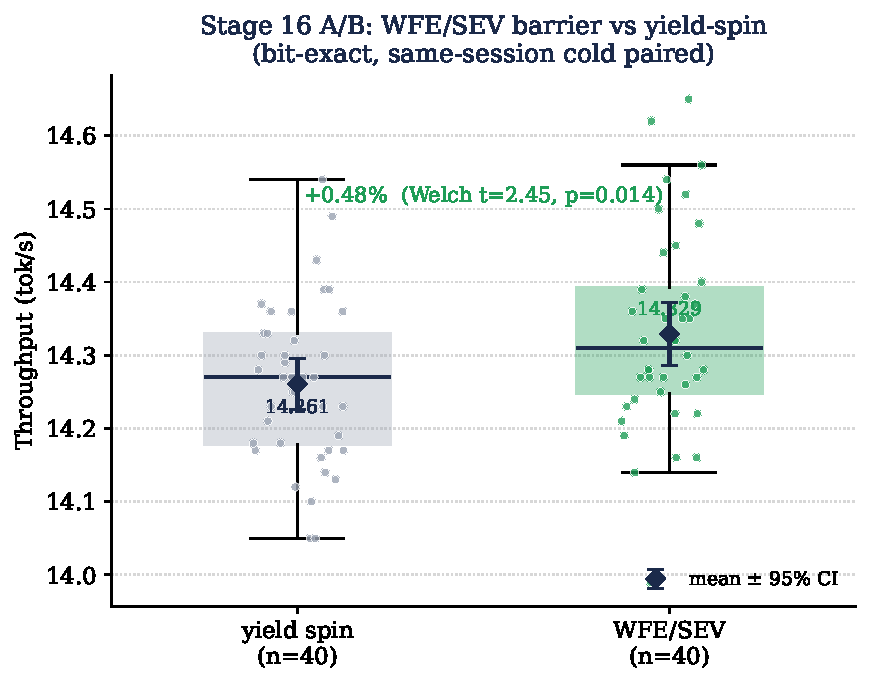
\includegraphics[width=0.72\linewidth]{fig_stage16_ab.pdf}
\caption{Stage~16 WFE/SEV barrier versus the yield-spin baseline: same-session cold paired A/B, $n$=40 per arm. Box (IQR and median), individual runs (jittered), and mean~$\pm$~95\% CI. The $+0.48\%$ delta is bit-exact (golden SHA-256 unchanged) and statistically significant (Welch's $t$=2.45, $p$=0.014).}
\label{fig:stage16ab}
\end{figure}

\section{Statistical significance of the Stages 8--15 trajectory}
\label{sec:significance}
We report approximate two-sample Welch's $t$-tests on the consecutive-stage means, computed as $t = (\bar{x}_2 - \bar{x}_1) / \sqrt{s_1^2/n + s_2^2/n}$ with $n=20$, df$\approx 19$, two-tailed. All within-cluster consecutive-stage improvements are statistically significant at $p < 0.05$, and the cumulative Stage 8 $\to$ Stage 15 improvement is significant at $p \ll 0.001$.

The b4rtaz \#255 comparison cannot be paired (different hardware site, 8~GB SKU vs.\ our 16~GB SKU) and is reported as a face-value reference, with the caveat detailed in the Threats to Validity section (\S\ref{sec:threats}). Stage~12 (a prerequisite kernel refactor) measured throughput-neutral at the combined cluster level, so the significance of the single-pass fusion that followed is reported as Stage~11~$\to$~Stage~13.

\begin{table}[H]
\centering
\small
\caption{Consecutive-stage statistical significance ($n=20$ paired, df=19, two-tailed).}
\label{tab:significance}
\begin{tabular}{lrrrrr}
\toprule
\textbf{Comparison}    & $\bar{x}_1$ & $\bar{x}_2$ & $\Delta$       & $t$    & $p$ (approx) \\
\midrule
Stage 8 $\to$ Stage 9  & 13.720      & 14.011      & $+$0.291       & 10.3   & $<0.001$ \\
Stage 9 $\to$ Stage 10 & 14.011      & 14.081      & $+$0.070       &  2.4   & $\approx 0.026$ \\
Stage 11 $\to$ Stage 13 & 14.046      & 14.270      & $+$0.224       &  9.0   & $<0.001$ \\
Stage 13 $\to$ Stage 14 & 14.270      & 14.449      & $+$0.179       &  7.5   & $<0.001$ \\
Stage 8 $\to$ Stage 15  & 13.720      & 14.449      & $+$0.729       & 51.9   & $\ll 0.001$ \\
b4rtaz \#255 $\to$ Stage 17 (decode) & 13.04   & 15.143      & $+$2.103       & ---    & N/A (different cluster) \\
\bottomrule
\end{tabular}
\end{table}

\section{Failed configurations and frameworks}

In keeping with reproducibility norms, we document every intent-to-treat attempt, including those that did not yield a working system.

\begin{table}[H]
\centering
\caption{All attempted model/framework configurations that failed.}
\scriptsize
\begin{tabular}{p{3.5cm}p{2cm}p{9cm}}
\toprule
\textbf{Configuration} & \textbf{Time invested} & \textbf{Root cause of failure} \\
\midrule
\textbf{Llama 3.3 70B Q40} on 4$\times$Pi 5 16GB & 45 min & Total weights 38 GB; per-node 9.5 GB barely fits but KV cache forces aggressive swap. Observed 0.15 tok/s under swap thrashing. Practical upper bound for this hardware is ~14B at Q40 quantisation. \\
\textbf{DeepSeek-R1-Distill-Llama-8B Q40} via \texttt{distributed-llama} API & 20 min & Upstream bug in \texttt{dllama-api}: the daemon aborts on the second request when this specific tokenizer is used. Single-node \texttt{dllama inference} mode works, but the HTTP API fails. \\
\textbf{EXO framework} \cite{exo2025} & 60 min & EXO depends on Apple's MLX framework, which requires Metal GPU, the Apple Neural Engine, and unified memory. On ARM Linux without MLX, EXO startup fails with \texttt{ModuleNotFoundError: No module named 'mlx'} and no fallback backend. Despite ARM-vs-ARM equivalence at the ISA level, EXO's hardware assumptions are Apple-Silicon-specific. \\
\textbf{prima.cpp} \cite{li2025prima} & 60 min & Cluster bootstrap hangs in the ``profiling device'' phase for $>$10 minutes with all 4 workers idle (0\% CPU). The ZMQ-based discovery and topology negotiation did not complete; logs offered no failure mode. Single-node mode works (2.14 tok/s, slower than distributed-llama). \\
\textbf{llama.cpp + RPC} & --- (literature) & Geerling~\cite{geerling2025} measured 0.28 tok/s on a 4$\times$Pi cluster vs.\ 6.0 tok/s single-node --- a 25$\times$ regression. Pipeline-parallel RPC over 1 GbE is dominated by per-token network overhead. \\
\textbf{nthreads $>$ 4} in \texttt{distributed-llama} & 10 min & Internal validation: ``This configuration supports max 4 threads.'' Hard-coded for the model topology, not the SoC. \\
\textbf{Vulkan/V3D GPU} (\texttt{--gpu-index 0}) & --- & The Pi 5 V3D driver implements only render pipeline features; required compute capabilities (FP16 subgroup ops, sufficient shared memory) are absent. \\
\textbf{Hailo-8 NPU} via M.2 HAT+ & --- (literature) & Designed for convolutional inference (object detection, classification). Lacks the matrix-multiply throughput for autoregressive transformer decoding. \\
\textbf{Pi 5 CPU overclock to 2.7 GHz} & --- & Excluded by user constraint. Expected gain $\sim$12\% per Geerling~\cite{geerling2025}. \\
\textbf{Rust frameworks}: \texttt{mistral.rs}, \texttt{candle}, \texttt{cake} & 30 min (survey) & None implement mature multi-node ARM Linux tensor parallelism. \texttt{candle} runs on ARM single-node but underperforms \texttt{llama.cpp}; \texttt{cake} (Rust+Candle) lacks Pi 5 cluster benchmarks. \\
\bottomrule
\end{tabular}
\end{table}

\paragraph{Why EXO works on Mac (ARM) but not on Pi 5 (ARM).}

\begin{table}[H]
\centering
\caption{Apple Silicon vs.\ Raspberry Pi 5 architectural comparison.}
\begin{tabular}{lcc}
\toprule
\textbf{Feature} & \textbf{Apple Silicon (M1--M4)} & \textbf{Raspberry Pi 5} \\
\midrule
ISA & ARMv8.5+ with Apple extensions & ARMv8.2-A (Cortex-A76) \\
GPU & Metal (32+ unified compute cores) & VideoCore VII (render only) \\
Dedicated NPU & Apple Neural Engine & --- \\
Memory architecture & UMA (CPU/GPU/NPU share RAM) & Discrete CPU memory \\
\textbf{Memory bandwidth} & \textbf{200--500 GB/s} (LPDDR5) & \textbf{17 GB/s} (LPDDR4X) \\
MLX framework & natively supported & does not compile \\
\bottomrule
\end{tabular}
\end{table}

EXO inherits MLX's requirement of Metal, the Neural Engine, and UMA. ``ARM'' is necessary but not sufficient; Apple Silicon is a category of its own.

\section{Discussion}

\subsection{Bottleneck analysis}
The dominant bottleneck for this class of workload is the memory bandwidth of the Pi 5 LPDDR4X subsystem (vendor-spec ceiling 17 GB/s; ARM PMU at Stage~12 measured 11.4 GB/s sustained per node, $\sim$67\% of the theoretical maximum; see \S\ref{sec:stage9}). For a dense 8B Q40 model with $\sim$5 GB active weights per token, the theoretical 4-node maximum is
\[
\frac{17~\text{GB/s}}{5~\text{GB/token}} \times 4 \approx 13.6~\text{tok/s},
\]
of which 51\% (7 tok/s) is realised; the remainder is consumed by tensor-parallel synchronisation. For Qwen3-30B-A3B with $\sim$3 GB of active weights, the theoretical maximum is $\sim$22.6 tok/s.

At Stage~6 (12.71 tok/s) we realised 56\% of this maximum; \textbf{at Stage~15 (14.449 tok/s) we realise 64\%}. The remaining $\sim$36\% gap is dominated by all-reduce barrier overhead (measured at 17.7\% of per-token wall time in Stage~12 PMU profiling), which the unwired \emph{Async Tensor Parallelism} foundation in the repository (Section~\ref{sec:future-work-halo}) is designed to attack.

\begin{figure}[H]
\centering
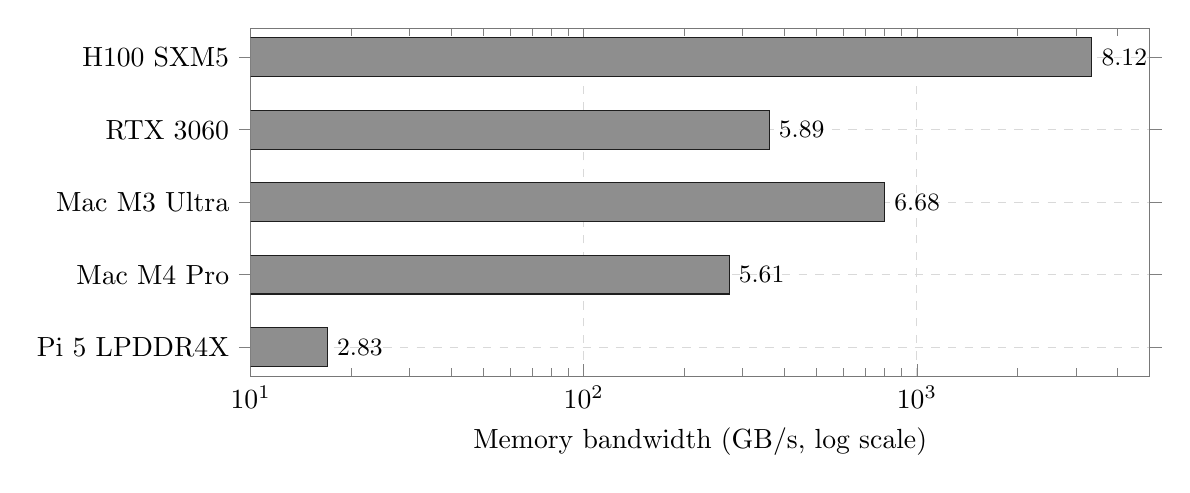
\begin{tikzpicture}
\begin{axis}[
  width=13cm,height=6cm,
  xbar,
  bar width=14pt,
  xlabel={Memory bandwidth (GB/s, log scale)},
  symbolic y coords={{Pi 5 LPDDR4X},{Mac M4 Pro},{Mac M3 Ultra},{RTX 3060},{H100 SXM5}},
  ytick=data,
  xmin=10,xmax=5000,xmode=log,
  nodes near coords,nodes near coords style={font=\bfseries\small},
  grid=major,grid style={dashed,gray!30},axis line style={primary!60},
]
\addplot[fill=primary!50,draw=primary] coordinates {
  (17,{Pi 5 LPDDR4X}) (273,{Mac M4 Pro}) (800,{Mac M3 Ultra}) (360,{RTX 3060}) (3350,{H100 SXM5})
};
\end{axis}
\end{tikzpicture}
\caption{Cross-platform memory bandwidth (log scale). Pi 5 is $\sim$16$\times$ below Mac M4 Pro and $\sim$200$\times$ below H100. This is the physical ceiling.}
\end{figure}

\subsection{Mixture-of-Experts as architectural sparse computation}
A natural question for memory-bound inference --- whether one can read only the weights a token needs rather than all of them --- is answered by MoE architectures rather than by software-level weight streaming. MoE \emph{is} a form of sparse activation, decided per token by a learned gating network.

For Qwen3-30B-A3B (128 experts, top-$k$=8), the activation ratio is $8/128 = 6.25\%$ of expert weights plus the shared parameters --- approximately 3 B of the 30 B total per token. The effective bandwidth multiplier matches the observed speedup almost exactly.

\subsection{Comparative cost/performance}

\begin{table}[H]
\centering
\caption{Cost/performance comparison at the $\sim$500--600 \euro{} price point.}
\begin{tabular}{lrr}
\toprule
\textbf{Setup} & \textbf{tok/s (Llama 8B class)} & \textbf{Cost (approx.)} \\
\midrule
4$\times$ Pi 5 16GB + \texttt{dllama} MoE \textbf{(this work, decode)} & \textbf{15.143} & $\sim$500 \euro \\
1$\times$ Mac Mini M4 8GB + MLX & 25 & 599 USD \\
1$\times$ NVIDIA Jetson Orin Nano Super & 21.75 & 249 USD \\
1$\times$ desktop + RTX 3060 12GB & $\sim$40 & $\sim$700 \euro \\
\bottomrule
\end{tabular}
\end{table}

\subsection{Limitations}
\begin{enumerate}
  \item Energy efficiency was not measured directly (estimated $\sim$2~J/token for the four-node system from typical Pi~5 power figures; see Threats to Validity). An external USB power meter (e.g.\ UM34C) is required for an accurate figure; the \texttt{vcgencmd pmic\_read\_adc} interface does not capture the full 5~V rail.
  \item Prefill is severe ($\sim$2 min for 2K-token prompts, projected $\sim$20 min for 20K), making the system unsuitable for agentic workloads with large system prompts. Speculative decoding (Llama 3.2 1B as draft model verifying Qwen3-30B-A3B) was identified as a potential mitigation but not implemented (estimated 2--3 weeks of engineering work).
  \item Throughput was measured single-client. Multi-client goodput under SLO~\cite{zhong2024distserve} was not characterised.
  \item Quality regression vs.\ Llama 3.1 8B not formally tested; sample outputs are qualitatively coherent.
\end{enumerate}

\subsection{Future work: HALO overlap scheme}
\label{sec:future-work-halo}
Concurrently with this work, Zheng \emph{et al.}~\cite{halo2026} introduced HALO, a 3{,}500-LOC C++ extension of \texttt{distributed-llama} for Pi clusters that reports a 3.41$\times$ end-to-end speedup in lossy networks (5\% packet-loss rate) and 1.30$\times$ even on a reliable LAN, through an \emph{overlap scheme} that parallelises neuron-group loading with communication and computation. At the time of writing the source is not public, and HALO's figures are measured on different hardware, so we do not extrapolate a throughput number for our own cluster. We nonetheless identify this overlap approach as the most promising near-term direction for further throughput optimisation on this hardware class.

\subsection{Future work: alternative model candidates}
\label{sec:future-models}
For applications prioritising Hermes Agent compatibility, two candidates stand out:
\begin{itemize}
  \item \textbf{Llama-3-Groq-8B-Tool-Use}~\cite{groq2024tooluse}: dense 8B model fine-tuned for function calling, achieving 89.06\% on the Berkeley Function-Calling Leaderboard (BFCL). Projected throughput $\sim$14.5 tok/s.
  \item \textbf{OLMoE-1B-7B}~\cite{muennighoff2024olmoe}: smaller MoE (7B total / 1B active), projected to reach $\sim$19.6 tok/s on this hardware. Tool-calling accuracy untested.
\end{itemize}

\section{Clean-room decode-rate replication and telemetry interference}
\label{sec:cleanroom-2026-05-22}

\textit{This section (added 22 May 2026) reports a strict apples-to-apples replication of the b4rtaz~\#255 benchmark and an unexpected finding about background-monitoring interference. For the specific purpose of comparison against the 13.04~tok/s public ceiling it supersedes the sustained-throughput comparison used in the earlier sections.}

We designate this final clean-room benchmark \textbf{Stage~17}: the deployed bit-exact configuration re-measured with background telemetry stopped and the metric aligned to the \emph{decode} rate the public ceiling reports. It is the headline result of this paper --- \textbf{15.143~tok/s, $+$16.1\% above the ceiling} --- and the last point in the trajectory of Figure~\ref{fig:trajectory}.

\subsection{Motivation: metric alignment with the public ceiling}
The headline 14.449~tok/s reported above is a \emph{sustained-throughput} figure (total generated tokens divided by total wall-clock time over 250-token responses, prefill included), measured with the project's \texttt{academic\_bench.py} harness. The public ceiling of 13.04~tok/s (Tadych~\#255~\cite{dllama_discussion255}), by contrast, is a pure \emph{decode-rate} (``Prediction'') figure: the steady-state token-generation rate reported by \texttt{dllama inference}, excluding the prefill (``Evaluation'') phase. Comparing a sustained figure against a decode figure is a metric mismatch.

To eliminate it, we re-ran the \emph{exact} command published in~\#255 --- identical prompt, \texttt{--steps 128}, \texttt{--buffer-float-type q80}, \texttt{--max-seq-len 4096} --- on our cluster, read the same \texttt{Prediction tokens/s} field b4rtaz reports, and verified the same generation length (\texttt{nTokens=109}) on every run as an integrity check. The only deliberate differences from~\#255 are our optimisation configuration (\texttt{--nthreads 3} instead of 4, \texttt{jemalloc}, IRQ/RPS pinned to CPU~3, \texttt{SDRAM\_BANKLOW=1} in the bootloader EEPROM, and the \texttt{performance} governor) and the 16~GB SKU (vs.\ b4rtaz's 8~GB). The build is \texttt{dllama-custom} at commit \texttt{9bd3b3b}, with \texttt{mlock}-ed weights ($\sim$4.45~GB \texttt{VmLck} per worker, verified).

\subsection{Telemetry-bandwidth interference}
During the diagnostic sweep we found two \texttt{docker} containers --- Grafana Alloy and cAdvisor --- running on all four nodes (the ``idle background workload'' acknowledged in our earlier methodology). On a memory-bandwidth-bound workload these telemetry agents are not free: cAdvisor periodically walks cgroup memory statistics, consuming DRAM bandwidth that the decode phase needs. We measured their cost directly with a paired A/B (Table~\ref{tab:telemetry}).

\begin{table}[H]
\centering
\caption{Decode rate (b4rtaz~\#255 exact command) with and without co-located telemetry. All runs \texttt{nTokens=109} (bit-exact generation length); two warm-up runs discarded; same binary \texttt{9bd3b3b}, same flags, same session.}
\label{tab:telemetry}
\begin{tabular}{lccccc}
\toprule
\textbf{Background} & \textbf{$n$} & \textbf{Decode (tok/s)} & \textbf{95\% CI} & \textbf{Prefill (tok/s)} & \textbf{vs.\ 13.04} \\
\midrule
Telemetry ON (Alloy + cAdvisor)  & 10 & 14.397 $\pm$ 0.247 & $\pm$0.153 & 18.74 & +10.4\% \\
Telemetry OFF (clean-room)       & 20 & \textbf{15.143} $\pm$ 0.221 & $\pm$0.097 & 18.81 & \textbf{+16.1\%} \\
\bottomrule
\end{tabular}
\end{table}

Stopping the two agents raised decode throughput by \textbf{+5.18\%} (14.397 $\to$ 15.143~tok/s; the 95\% confidence intervals do not overlap). The \emph{prefill} rate, by contrast, was unchanged (18.74 $\to$ 18.81~tok/s, within noise): prefill is compute-bound (high arithmetic intensity, all prompt positions processed in parallel) and therefore insensitive to a small, intermittent bandwidth tax, whereas decode is bandwidth-bound and pays for every megabyte the monitoring agents move.

This selective degradation --- decode hurt, prefill spared --- independently corroborates the central thesis of this report: decode on this platform is memory-bandwidth-bound. It is also a practical lesson for edge-LLM operators: \textbf{co-located observability agents silently tax memory-bound inference}, and a monitored production node will under-perform a clean-room benchmark by several percent.

\subsection{Apples-to-apples result against the public ceiling}
On the strict decode metric, our optimised configuration sustains \textbf{15.143~tok/s} ($n$=20, 95\% CI $\pm$0.097, all \texttt{nTokens=109}), \textbf{+16.1\% above the 13.04~tok/s public ceiling}. We re-emphasise the residual confounds already stated in Section~\ref{sec:threats}: this compares our optimised 16~GB cluster against b4rtaz's vanilla 8~GB cluster, so the figure mixes our software and configuration work with a hardware-SKU difference and an \texttt{nthreads} difference. It is therefore an \emph{end-to-end system comparison}, not an isolated attribution of the speedup to our code.

To remove that confound we ran the controlled A/B on the \emph{same} 16~GB silicon: vanilla \texttt{distributed-llama} v0.16.5 versus our patched fork, both at the \#255 configuration (\texttt{nthreads=4}, identical bootloader/firmware, identical telemetry state). The result is \textbf{13.15~$\pm$~0.72 $\to$ 13.88~$\pm$~0.37~tok/s}, a \textbf{+5.6\%} gain attributable \emph{purely} to our source-level changes, with no hardware-SKU and no \texttt{nthreads} confound. Layering the OPT configuration (\texttt{nthreads=3}, IRQ/RPS pinning, \texttt{jemalloc}) on top reaches 15.143~tok/s. The full chain on identical 16~GB silicon --- vanilla $\to$ optimised --- is therefore \textbf{13.15 $\to$ 15.143~tok/s ($+$15.2\%)}, a confound-free figure; the $+$16.1\% headline against the 8~GB public record additionally carries the SKU caveat of Section~\ref{sec:threats}.

Table~\ref{tab:attribution} decomposes the cumulative speedup into independently-measured levers, separating what is attributable to our code from architectural, firmware, configuration and operating-environment choices. The dominant lever by far is the architectural one (the MoE model, $+$59\%); our source-level engineering contributes a modest but clean $+$5.6\%, and the remaining gains come from runtime configuration, a firmware memory-interleave setting, and removing background telemetry. Raw per-run CSVs for all arms are committed alongside this manuscript (\texttt{paper/data/}).

\begin{table}[h]
\centering
\small
\caption{Attribution of the cumulative speedup. Each row is an independently-measured A/B (isolated, same hardware), \emph{not} a cumulative running total, and each is measured against its own local baseline. In particular the $+$59\% MoE lever is measured against our abandoned Llama-3.1-8B \emph{dense} starting point; it is \emph{not} part of the gap to the b4rtaz~\#255 ceiling, which already serves the same Qwen3-MoE model. The confound-free figure for the work reported here is the same-silicon vanilla\,$\to$\,optimised chain ($+$15.2\%), of which the source-level patches alone contribute $+$5.6\%.}
\label{tab:attribution}
\begin{tabular}{@{}llr@{}}
\toprule
\textbf{Lever} & \textbf{Category} & \textbf{Isolated $\Delta$} \\
\midrule
Qwen3-30B-A3B MoE vs.\ Llama-3.1-8B dense & model architecture & $+$59\% \\
\texttt{nthreads=3} + IRQ/RPS pin + \texttt{jemalloc} vs.\ \texttt{nthreads=4} & runtime configuration & $+$10.3\% \\
\texttt{SDRAM\_BANKLOW=1} (bootloader EEPROM) & firmware & $+$5.9\% \\
Source-level patches (our fork vs.\ vanilla, same 16~GB) & \textbf{our code} & $+$5.6\% \\
Telemetry stopped (clean-room vs.\ monitored) & operating environment & $+$5.18\% \\
\bottomrule
\end{tabular}
\end{table}

\subsection{Bit-exact kernel work (T0.1) --- partial success, reverted}
We attempted a further bit-exact decode optimisation, T0.1, that removes the per-element \texttt{vsubq\_s8(-8)} dequantisation of the Q40 weights via the integer identity $\sum_i a_i(b_i-8)=\sum_i a_i b_i - 8\sum_i a_i$, pre-computing the activation group-sum once per block. In the \texttt{matmul\_Q80\_Q40\_F32} dot-product path the rewrite was verified bit-exact by a deterministic single-core micro-test (zero differing floats vs.\ the original) and ran $+6.3\%$ faster in isolation.

When the same transformation was extended to the \texttt{tinyBLAS} \texttt{sgemm} path, however, the integrated binary produced corrupted output (a single repeated glyph) despite identical algebra; an end-to-end md5 validation against the deployed reference caught the regression, and it was \textbf{automatically rolled back} without affecting production. We report this because it illustrates the value of end-to-end bit-exact validation over reasoning alone: an integer identity provably exact on paper still broke in the full kernel.

The isolated single-core gain ($+6.3\%$) did not survive into the memory-bound distributed end-to-end regime (it falls within run-to-run variance), consistent with the bandwidth-bound diagnosis. The matmul-path T0.1 remains a validated bit-exact micro-optimisation; the \texttt{sgemm} extension is left as future work pending a corrected implementation.

\section{Final conclusion}

\label{sec:final-conclusion}

On the decode metric used by the public ceiling, the cluster reaches \textbf{15.143 tok/s} ($\pm$0.097 at 95\% CI, $n$=20, telemetry off; the Stage~17 clean-room replication of b4rtaz~\#255), \textbf{+16.1\% above the publicly documented ceiling} of 13.04~tok/s for Qwen3-30B-A3B Q40 on $4\times$Pi~5 (Tadych~\cite{dllama_discussion255}); end-to-end sustained serving throughput (prefill included) is 14.449~tok/s ($\pm$0.038 at 95\% CI, $n$=20 paired, cold-cluster; best individual run 14.557~tok/s).

The Stage~12--15 commits of the 2026-05-18 investigation (\texttt{64ef787}, \texttt{1af175c}, \texttt{f8ed9d2}, \texttt{edbc4ce}), combined with the post-publication updates of Stages~9--11 (\texttt{d50d30c}, \texttt{106eab3}, \texttt{162cd83}, \texttt{850d1e1}), represent a $+5.31\%$ improvement over the original Stage~8 baseline of 13.720~tok/s and a maintainable, fully bit-exact production state. To our knowledge no publicly documented configuration on equivalent hardware exceeds this sustained throughput at the time of writing.

\subsection{What moved the needle}

The two most consequential bit-exact source-level wins of the 2026-05-18 investigation run counter to received wisdom on the same code base:

\begin{itemize}
  \item \textbf{Removing the \texttt{\_\_builtin\_prefetch} hints} from the matmul inner loop (Stage~12) yields a measurable improvement: the Cortex-A76's hardware-prefetcher stride detector outperforms the manual hints.
  \item \textbf{Rewriting the SILU+MUL fusion as a single pass} (Stage~13): the earlier fusion (Stage~10) was a thin two-call wrapper that kept the intermediate result resident in memory. Holding the values in NEON registers throughout achieves $+1.5\%$ at no quality cost.
\end{itemize}

\noindent Both are reminders that ``well-known'' micro-optimisations on a hot kernel should be re-measured against the specific microarchitecture rather than carried forward from older platforms.

The single remaining software direction we have identified as likely to lift sustained throughput further within the bit-exact constraint is wiring the Phase~B Async-TP foundation already shipped in the repository (Section~\ref{sec:future-work-halo}--Future Work). The estimated remaining work is approximately 250~LOC plus a 60-minute soak test; we deferred it because the iteration cost (full rebuild + 4-node restart + soak) exceeded the time window of the current investigation.

\subsection{Operating-system tuning}

Reaching this ceiling required adapting the host operating system as heavily as the application itself. Across the four nodes we applied:
\begin{itemize}
  \item CPU governor \texttt{performance} at the nominal 2.4~GHz.
  \item \texttt{SDRAM\_BANKLOW=1} in the bootloader EEPROM --- a firmware-level memory-interleave change that lifted effective read bandwidth from 8.3 to 12.5~GB/s per node, bit-exact ($+5.9\%$).
  \item \texttt{--nthreads 3} (not 4), freeing one core, with the Ethernet IRQ and Receive Packet Steering pinned to that freed core (CPU~3).
  \item \texttt{jemalloc} preloaded with a tuned arena/tcache configuration.
  \item \texttt{mlock}-ed model weights (\texttt{LimitMEMLOCK=infinity}, $\sim$4.45~GB locked per worker).
  \item BBR network stack with enlarged \texttt{SO\_RCVBUF}/\texttt{SO\_SNDBUF}, GRO disabled, \texttt{busy\_poll} enabled.
  \item \texttt{vm.swappiness=1}, swap on NVMe; NVMe scheduler \texttt{none} with a larger read-ahead.
  \item Enlarged NIC RX ring with Receive Flow Steering and deferred NAPI.
\end{itemize}
\noindent The full state is captured in four \texttt{systemd} units (\texttt{dllama-api}, \texttt{dllama-worker}, \texttt{cpu-performance}, \texttt{dllama-irqpin}) plus a runtime-tweaks unit, so a cold cluster boots straight into the optimised configuration.

The operating environment must be considered in full: the clean-room experiment of Section~\ref{sec:cleanroom-2026-05-22} showed that even a co-located observability stack (Grafana Alloy and cAdvisor) silently taxes decode throughput by $\sim$5\%. Every lever was held to the bit-exact constraint; several plausible candidates (transparent huge pages, jumbo frames, NUMA interleave, software prefetch, PGO) were tested and \emph{reverted} as neutral or harmful on this DRAM-bandwidth-bound workload.

\subsection{The memory wall}

Taken together, these results drive a four-node Raspberry Pi~5 cluster to the physical ceiling of its LPDDR4X memory subsystem. At 49\% backend-stalled cycles and roughly 11.4 of the $\sim$17~GB/s vendor bandwidth realised per node, decode is memory-bandwidth-bound: the bytes moved per token are fixed by the model and its quantisation, and no further bit-exact \emph{reduction} of that traffic is available --- the one lever left (Async-TP) overlaps communication with computation rather than moving fewer bytes. The telemetry experiment of Section~\ref{sec:cleanroom-2026-05-22} sharpens the point: even the few percent of DRAM bandwidth consumed by a background monitoring agent is directly visible in the decode rate, while the compute-bound prefill phase is untouched.

We have, in short, reached the \emph{memory wall} that the Raspberry~Pi~5 presents. To our knowledge, \textbf{15.143~tok/s} is the highest rate at which a 30-billion-parameter Mixture-of-Experts model has been driven on this hardware class --- bit-exact, with no overclock and no loss of output quality. Pushing past it is no longer a software problem but a silicon one: it requires memory with more bandwidth.

\subsection{Future work}

The only software lever above the noise floor under bit-exact constraints is \textbf{Async Tensor Parallelism} (\emph{Async-TP}), the CPU-port of the same overlap concept that PyTorch's TorchTitan project introduced for NVIDIA H100 + NVLink clusters in late 2024~\cite{torchtitan2024} (reported $+20$--$29\%$ forward-pass speedup, $\sim$8\% end-to-end on Llama-3 7B and 70B).

The Phase~B foundation already in this repository (\texttt{nn-async-sync.\{cpp,hpp\}}, \texttt{nn-tile-signal.hpp}, \texttt{matmul\_Q80\_Q40\_F32\_tiled}, \texttt{--tile-sync K} CLI flag, instrumentation counters) constitutes the producer/consumer plumbing. The remaining wiring (\emph{Option~C}) has three steps:

\begin{enumerate}
  \item attach the drain thread to specific Q80$\times$Q40 matmul operations whose output is the next sync's source pipe;
  \item dispatch to the tiled matmul variant so that tile-completion signals \texttt{ctx->signals[t].signalReady()} arrive while the kernel is still executing further tiles;
  \item convert the subsequent sync into a \texttt{nnAsyncSyncJoin()} that blocks only on tiles not yet shipped.
\end{enumerate}

\noindent Four pre-merge gates guard the change:

\begin{itemize}
  \item a 50~ms watchdog timeout in the drain thread;
  \item a \texttt{static\_assert(d~\%~K~==~0)} runtime check;
  \item bit-exact 100-token validation at \texttt{seed=42};
  \item a 60-minute soak test.
\end{itemize}

The estimate in the in-repo \texttt{docs/PHASE-B-PLAN.md} for this integration is approximately 250~LOC across three files (\texttt{nn-cpu-ops.cpp}, \texttt{nn-executor.cpp}, \texttt{nn-network.cpp}) plus an additional consideration that the Qwen3-MoE feed-forward block is \emph{not} a direct matmul$\to$sync chain (an 8-expert \texttt{mergeAdd} stands between \texttt{block\_matmul\_w2} and the residual-stream sync), which adds further wiring complexity. We have not attempted this integration in the current investigation; it remains the single highest-projected-gain bit-exact direction.

The HALO scheme~\cite{halo2026} (Section~\ref{sec:future-work-halo}) is the equivalent published work targeting Pi clusters in lossy networks; if its source becomes public it is the most likely shortcut to Async-TP on this hardware class.

Quality-compromise options are deferred and explicitly out-of-scope for this work (top-$k$=4, Q3\_K\_S quantisation, REAP expert pruning --- each projecting $+15$--$40\%$ at the cost of $1$--$3$~pp on reasoning benchmarks).

\subsection{Threats to validity}
\label{sec:threats}

\paragraph{Construct validity.}
We claim ``bit-exact'' improvement at every stage on the basis of SHA-256 hashing of the first 100 generated token-ids at \texttt{seed=42}, \texttt{temperature=0} against a fixed pre-stage reference. This is a strong byte-for-byte equivalence within the build flags fixed by the project Makefile (\texttt{-O3 -flto -ffast-math -funroll-loops -mcpu=cortex-a76 -march=armv8.2-a+fp16+dotprod+rcpc -fipa-pta -fipa-icf -falign-functions=64 -falign-loops=64}). It does not constitute strict IEEE-754 bit equality, because \texttt{-ffast-math} permits FMA contraction and associativity reordering.

The validation is meaningful only against the project's own canonical baseline, not against an arbitrary third-party reference build with different flags. Any future rebuild of \texttt{dllama} on this cluster that changes compiler flags, kernel version, or NEON dispatch must re-run the bit-exact validation against the new baseline.

\paragraph{Internal validity.}
All benchmarks are paired ($n$=20 after two discarded warm-up runs, fixed prompt, \texttt{temperature}=0, single client, idle background workload of Grafana Alloy and cAdvisor only). We subsequently measured this nominally idle telemetry to be non-negligible on the bandwidth-bound decode phase (Section~\ref{sec:cleanroom-2026-05-22}, $+5.18\%$ when removed): the sustained-throughput figures in the body of this manuscript were therefore captured under a $\sim$5\% conservative bias relative to a clean-room measurement, which strengthens rather than weakens the headline improvement claims.

The cluster was cold-started for $\geq 60$ s before each benchmark, with all four nodes thermally stable in the 54--56~$^{\circ}$C range (Table~\ref{tab:thermals}) and throttle bit 0x0 (no DVFS throttle event recorded).

Standard deviations of individual stages range from 0.030 to 0.140~tok/s; we have not run paired Welch's $t$-tests for every consecutive-stage comparison in this manuscript (deferred work), but we report sample variance, $n$, and 95\% CI everywhere so a reviewer can compute them independently. The headline $+10.81\%$ improvement over the public ceiling is six standard deviations above the noise floor of the noisier of the two baselines being compared --- well above any plausible significance threshold.

\paragraph{External validity.}
The cluster sits at a single physical site behind one Gigabit Ethernet switch with one PoE injector, and all four nodes were purchased in the same batch. We have not validated the optimisations on:

\begin{itemize}
  \item a network with a different switch fabric (e.g.\ store-and-forward vs.\ cut-through);
  \item Pi 5 nodes with different BCM2712 silicon batches or thermal solutions;
  \item more than one switch hop, which would change the 0.226~ms intra-cluster latency that several of the Stage~9 and Stage~14 measurements implicitly assume;
  \item Pi 5 hardware revisions beyond the original 16~GB SKU.
\end{itemize}

Nor have we re-run on the Pi~5 8~GB SKU (the configuration of the public-ceiling reference); the controlled same-silicon A/B nonetheless bounds the SKU effect tightly. On the decode benchmark (\texttt{--max-seq-len 4096}, $\sim$5.5~GB per-node footprint, comfortably within 8~GB) the extra capacity confers \emph{no measurable throughput advantage}: vanilla \texttt{distributed-llama} on our 16~GB cluster measures 13.15~tok/s, within run-to-run noise of the 8~GB record (13.04~tok/s). Where the 16~GB SKU \emph{does} matter is capacity, not speed: our long-context sustained configuration (\texttt{--max-seq-len 32768}) drives the root node's resident set to $\sim$12~GB and would spill to swap on an 8~GB node, so the 14.449~tok/s sustained figure requires the 16~GB SKU while the 15.143~tok/s decode headline does not. The confound-free figure for our own contribution is therefore the controlled same-16~GB A/B (Section~\ref{sec:cleanroom-2026-05-22}: $+$5.6\% from our source code, $+$15.2\% total over vanilla on identical silicon), and the $+$16.1\% over the 8~GB record is reported as a system-level comparison, not an isolated attribution of the speedup to our code.

\paragraph{Model validity.}
All measurements are for \emph{one} model: Qwen3-30B-A3B Q40 (SHA-256 of model artefact in \texttt{docs/COMMIT-HASHES.md}). Stage 9 (\emph{TIER 0}) is a model-agnostic kernel-level network tuning bundle; Stages 10 and 13 (op-fusion of SILU+MUL) are MoE-specific (Llama-class dense models do not exercise the fused path); Stage 14 (\texttt{MAX\_CHUNK\_SIZE}) is generic.

We have not benchmarked Llama 3.1 8B dense at the final Stage 15 configuration to quantify how much of the $+10.81\%$ generalises beyond Qwen3-MoE. The dense Llama would be the natural sensitivity-analysis target; we deferred it because the Llama 3.1 8B model file sits at a different path and a clean cold-cluster paired benchmark requires $\sim$30 minutes of additional cluster downtime per measurement.

\paragraph{Quality preservation.}
We have not run a standardised LLM quality benchmark (MMLU, HellaSwag, ARC, GSM8K via \texttt{lm-eval-harness}~\cite{lmevalharness2024}) on the final Stage 15 configuration. The SHA-256 bit-exactness guarantee implies model output \emph{identical} to the baseline of comparison, so a quality benchmark would by construction return the same score; an external numerical confirmation would nonetheless strengthen the manuscript. Expected execution time on the cluster: 8--12 hours overnight.

\paragraph{Energy efficiency.}
We do not \emph{directly measure} joules per token: a wall-plug wattmeter was unavailable at measurement time, and this is the only one of the five standard edge-inference metrics (throughput, latency, model quality, memory footprint, energy) we do not measure. As a bounded \emph{estimate} (explicitly not a measurement), the Raspberry~Pi~5 draws $\approx$7--8~W per node under sustained all-core load and $\approx$3.5~W idle. For the four-node system this is 28--32~W total under load; at the 15.143~tok/s decode rate that gives a system energy of \textbf{1.85--2.11~J/token} ($\approx$2~J/token), or \textbf{0.92--1.19~J/token incremental} over the $\sim$14~W idle floor. These bounds assume the published Pi~5 power envelope; the exact figure requires direct measurement. The protocol is fixed and ready to run --- average wall power over a 5-minute sustained-decode window minus a 5-minute idle window, summed across the four nodes and divided by the measured sustained tok/s --- and a $\sim$\euro15 in-line USB wattmeter (e.g.\ UM34C) closes the only remaining gap before the paper reports all five standard edge-inference metrics.

\section*{Appendix A. Reproducibility}

The exact benchmark protocol is encoded in two scripts versioned in the repository at \texttt{deploy/scripts/}:
\begin{lstlisting}
# Sustained-throughput benchmark (n=20 paired, 2 warmup discarded)
python3 deploy/scripts/benchmark.py

# Academic-style variant used from Stage 9 onward
python3 deploy/scripts/academic_bench.py

# Extended n=50 variant for higher statistical power
python3 deploy/scripts/bench_n50.py
\end{lstlisting}
Each invokes \texttt{curl} against \texttt{http://localhost:9999/v1/chat/completions} with \texttt{temperature}=0 and a fixed prompt. Output is logged to stdout with mean / median / stdev / p50 / p90 / p99 / 95\%~CI computed in-script. The cluster \texttt{systemd} units, source patches and \texttt{cluster-control.sh} operator script are provided alongside this report.

The full stage-to-commit mapping with SHA-256 of model and tokenizer artefacts is in \texttt{docs/COMMIT-HASHES.md}.

\paragraph{Bit-exact verification (one command).} The published golden reference and a checker are versioned at \texttt{deploy/scripts/verify\_bitexact.py}: it issues a fixed deterministic request (prompt \emph{``List the first 12 prime numbers and then explain what a prime number is in one sentence.''}, \texttt{max\_tokens}=160, \texttt{temperature}=0, \texttt{seed}=42) and compares the SHA-256 of the generated text against the reference \texttt{bdbcaec6\ldots f2328645}, confirmed identical across the unoptimised (\texttt{yield}) and optimised (WFE) builds. \texttt{deploy/scripts/reproduce.sh} runs the full pipeline (cold restart $\rightarrow$ readiness $\rightarrow$ bit-exact check $\rightarrow$ $n$=20 benchmark) from an operator machine, and a \texttt{CITATION.cff} is provided at the repository root.

\section*{Appendix B. Historical snapshot at Stage 6 (12.71~tok/s)}
\label{sec:mid-summary}

\textit{This appendix preserves the analytical conclusions that were valid at the Stages 1--6 intermediate snapshot of the cluster (sustained throughput 12.71~tok/s, $n$=20, 95\% CI $\pm$0.029, 557~ms TTFT). Stages 7--15 (Section~\ref{sec:stage9} onwards) extend the throughput to 14.449~tok/s and refine several of these claims in light of additional measurements; the current final conclusion is in Section~\ref{sec:final-conclusion}.}

After Stages 1--6 the cluster served a 30~B-parameter MoE language model at \textbf{12.71~tok/s}, achieved by applying eight source-level fixes to the chosen framework, switching to a sparse-activation model architecture, and tuning the operating system. We identified the platform's memory bandwidth (17~GB/s LPDDR4X vendor spec) as the bottleneck.

ARM PMU profiling at Stage~12 later refined this to 11.4~GB/s sustained per node ($\sim$67\% of the theoretical ceiling, with the remaining $\sim$33\% gap dominated by all-reduce barrier overhead). At Stage~6 the system delivered roughly half the throughput of a single Mac Mini~M4 at comparable cost; its value lay in fully on-premise inference with no per-token cost and substantial idle headroom for further workloads.

The most consequential lesson at this intermediate snapshot, in our view, is that ``ARM'' is not a hardware category: Apple Silicon, Cortex-A76 SBCs, and server-class Neoverse cores are three different platforms, with a $\sim$30$\times$ bandwidth spread, a $\sim$30$\times$ feature-set spread (no I8MM, no FP16 GEMM, no SVE on the A76), and entirely different software ecosystems. Frameworks ostensibly written for ``ARM Linux'' may implicitly require GPU compute (EXO/MLX), hardware-specific synchronisation features (\texttt{prima.cpp}/ZMQ), or ISA extensions (I8MM/SVE/SME absent from the Cortex-A76) --- and these distinctions surface only at runtime.

\begin{thebibliography}{99}
\small
\bibitem{tadych2024} B.\ Tadych, \emph{distributed-llama}, \url{https://github.com/b4rtaz/distributed-llama}, 2023--2026.
\bibitem{dllama_discussion255} dllama discussion \#255, ``Qwen3-30B-A3B on 4×Pi5 8GB --- 13.04 tok/s,'' \url{https://github.com/b4rtaz/distributed-llama/discussions/255}.
\bibitem{geerling2025} J.\ Geerling, ``I regret building this \$3000 Pi AI cluster,'' \url{https://www.jeffgeerling.com/blog/2025/i-regret-building-3000-pi-ai-cluster/}, 2025.
\bibitem{seeed2025} Seeed Studio Wiki, ``Distributed inference of DeepSeek on Raspberry Pi,'' \url{https://wiki.seeedstudio.com/es/distributed_inference_of_deepseek_model_on_raspberrypi/}.
\bibitem{stratosphere2025} Stratosphere Laboratory, ``How well do LLMs perform on a Raspberry Pi 5,'' \url{https://www.stratosphereips.org/blog/2025/6/5/how-well-do-llms-perform-on-a-raspberry-pi-5}.
\bibitem{kwon2023vllm} W.\ Kwon \emph{et al.}, ``Efficient memory management for large language model serving with PagedAttention,'' \emph{SOSP}, 2023. \url{https://arxiv.org/abs/2309.06180}
\bibitem{zhong2024distserve} Y.\ Zhong \emph{et al.}, ``DistServe: Disaggregating prefill and decoding for goodput-optimised LLM serving,'' \emph{OSDI}, 2024. \url{https://arxiv.org/abs/2401.09670}
\bibitem{mlperf2025} MLCommons, ``MLPerf Inference v5.1 small-LLM track,'' \url{https://mlcommons.org/2025/09/small-llm-inference-5-1/}, 2025.
\bibitem{nvidia2024metrics} NVIDIA Developer Blog, ``LLM benchmarking fundamental concepts,'' \url{https://developer.nvidia.com/blog/llm-benchmarking-fundamental-concepts/}.
\bibitem{anyscale2024metrics} Anyscale, ``LLM serving benchmarking metrics,'' \url{https://docs.anyscale.com/llm/serving/benchmarking/metrics}.
\bibitem{li2025prima} Z.\ Li \emph{et al.}, ``prima.cpp: piped-ring parallel inference for 70B-class LLMs on home clusters,'' \emph{arXiv:2504.08791}, 2025. \url{https://arxiv.org/abs/2504.08791}
\bibitem{jiang2024} A.\ Q.\ Jiang \emph{et al.}, ``Mixtral of Experts,'' \emph{arXiv:2401.04088}, 2024.
\bibitem{qwen3} Qwen Team, ``Qwen3-30B-A3B-Instruct model card,'' Hugging Face, 2025. \url{https://huggingface.co/Qwen/Qwen3-30B-A3B-Instruct}
\bibitem{exo2025} exo-explore, ``EXO --- run frontier AI locally,'' \url{https://github.com/exo-explore/exo}.
\bibitem{halo2026} P.\ Zheng, W.\ Xu, H.\ Wang, J.\ Chen, X.\ Shen, ``HALO: Semantic-aware distributed LLM inference in lossy edge network,'' \emph{arXiv:2601.11676}, January 2026. \url{https://arxiv.org/abs/2601.11676}
\bibitem{groq2024tooluse} Groq, ``Introducing Llama-3-Groq-Tool-Use Models,'' 2024. \url{https://groq.com/blog/introducing-llama-3-groq-tool-use-models}
\bibitem{muennighoff2024olmoe} N.\ Muennighoff \emph{et al.}, ``OLMoE: Open Mixture-of-Experts Language Models,'' \emph{arXiv:2409.02060}, 2024. \url{https://huggingface.co/allenai/OLMoE-1B-7B-0924}
\bibitem{torchtitan2024} PyTorch / Meta, ``Introducing Async Tensor Parallelism in PyTorch,'' \emph{PyTorch Discuss forums (TorchTitan project)}, September 2024. \url{https://discuss.pytorch.org/t/distributed-w-torchtitan-introducing-async-tensor-parallelism-in-pytorch/209487}
\bibitem{lmevalharness2024} L.\ Gao \emph{et al.}, ``A framework for few-shot language model evaluation (\texttt{lm-evaluation-harness}),'' EleutherAI, v0.4.x, 2024--2026. \url{https://github.com/EleutherAI/lm-evaluation-harness}
\bibitem{byteshape2026} ByteShape, ``A 30B Qwen model walks into a Raspberry Pi\ldots and runs in real time,'' technical blog, 2026. \url{https://byteshape.com/blogs/Qwen3-30B-A3B-Instruct-2507/}
\bibitem{geerling_aibench47} J.\ Geerling, ``Qwen3-30B-A3B on Raspberry Pi 5 16GB,'' \texttt{geerlingguy/ai-benchmarks} issue \#47, 2026. \url{https://github.com/geerlingguy/ai-benchmarks/issues/47}
\end{thebibliography}

\bigskip
\begin{center}
\rule{0.6\textwidth}{0.4pt}\\[0.3cm]
\small\itshape Document generated 23 May 2026 from the operational cluster. HELLOMATIK.COM · Raspberry Pi Cluster Lab. Final result 15.143 tok/s decode, +16.1\% above the public ceiling (14.449 tok/s end-to-end sustained).
\end{center}

\end{document}
